% ulm-lam-companion.tex -- a companion to "Modern Compiler Concepts: A Field
% Guide" that connects its theory with the implementation of ulm.lam.
% Build: latexmk (LuaLaTeX, see latexmkrc).  The examples: examples/run.sh.
\documentclass[11pt,a4paper,openany]{book}
% preamble.tex -- shared preamble of ulm-lam-companion.tex (LuaLaTeX)

\usepackage[a4paper,inner=2.6cm,outer=2.4cm,top=2.6cm,bottom=2.8cm,headheight=14pt]{geometry}

% ---------------------------------------------------------------- fonts
\usepackage{amsmath}
\usepackage{fontspec}
\usepackage{unicode-math}
\setmainfont{Libertinus Serif}
\setsansfont{Libertinus Sans}
\setmathfont{Libertinus Math}
\setmonofont{JuliaMono}[Scale=MatchLowercase]

% ------------------------------------------- paragraphs: no indent, \medskip
\usepackage[skip=\medskipamount]{parskip}

% ---------------------------------------------------------------- packages
\usepackage[dvipsnames]{xcolor}
\usepackage{microtype}
\usepackage{booktabs,tabularx,array,xltabular}
\usepackage{enumitem}
\usepackage{needspace}
\usepackage{listings}
\usepackage[most]{tcolorbox}
\usepackage{tikz}
\usetikzlibrary{positioning,arrows.meta,fit,calc,backgrounds,decorations.pathreplacing}
\usepackage{titlesec}
\usepackage{fancyhdr}
\usepackage[hyphens]{url}
\usepackage[unicode,bookmarksnumbered,linktoc=all]{hyperref}
\usepackage[nameinlink,capitalise,noabbrev]{cleveref}

\definecolor{accent}{HTML}{1F5A96}
\definecolor{metacolor}{HTML}{555555}
\definecolor{bg}{gray}{0.95}      % code blocks
\definecolor{ttbg}{gray}{0.92}    % inline typewriter text
\definecolor{theorybg}{HTML}{EAF2FB}
\definecolor{limitbg}{HTML}{FBF0E6}
\definecolor{kw}{HTML}{1F4E9A}
\definecolor{cm}{HTML}{6B6B6B}
\definecolor{ty}{HTML}{2E6B30}
\definecolor{st}{HTML}{8A3B12}
\hypersetup{colorlinks=true,linkcolor=accent,urlcolor=accent!70!black,citecolor=accent,
  pdftitle={ulm.lam and the Field Guide: A Companion},pdfauthor={}}

\setlist{itemsep=2pt,topsep=3pt,parsep=0pt}
\renewcommand{\arraystretch}{1.18}
\emergencystretch=3em
\raggedbottom

% ---------------------------------------------------------------- headings
\titleformat{\chapter}[display]
  {\sffamily\bfseries\huge\raggedright}
  {\large\color{accent}\MakeUppercase{\chaptertitlename}~\thechapter}{0.4em}{}
\titlespacing*{\chapter}{0pt}{0pt}{1.8em}
\titleformat{\section}
  {\sffamily\bfseries\Large\raggedright}{\color{accent}\thesection}{0.8em}{}
\titlespacing*{\section}{0pt}{2.0em plus 0.5em minus 0.3em}{0.5em}
\titleformat{\subsection}
  {\sffamily\bfseries\large\color{accent!85!black}\raggedright}{\thesubsection}{0.6em}{}
\titlespacing*{\subsection}{0pt}{1.2em plus 0.3em}{0.3em}
\titleformat{\paragraph}[runin]{\sffamily\bfseries}{}{0pt}{}[.]
\titlespacing*{\paragraph}{0pt}{0.6em}{0.5em}
\setcounter{secnumdepth}{2}
% a run-in heading that ends in its own punctuation (a question)
\newcommand{\qparagraph}[1]{\par\addvspace{0.6em}\noindent{\sffamily\bfseries #1}\enspace}
\setcounter{tocdepth}{1}

% ---------------------------------------------------------------- header
\pagestyle{fancy}
\fancyhf{}
\fancyhead[LE]{\small\sffamily\leftmark}
\fancyhead[RO]{\small\sffamily\rightmark}
\fancyfoot[C]{\small\sffamily\thepage}
\renewcommand{\headrulewidth}{0.3pt}
\renewcommand{\chaptermark}[1]{\markboth{\thechapter.\ #1}{}}
\renewcommand{\sectionmark}[1]{\markright{\thesection\ #1}}
\fancypagestyle{plain}{\fancyhf{}\fancyfoot[C]{\small\sffamily\thepage}\renewcommand{\headrulewidth}{0pt}}

% ---------------------------------------------------------------- inline code
% Grey background behind \texttt via lua-ul leaders: line spacing unchanged,
% line breaks still possible.
\usepackage{luacolor,lua-ul}
\NewCommandCopy{\origtexttt}{\texttt}
\DeclareRobustCommand{\texttt}[1]{\highLight[ttbg]{\origtexttt{#1}}}
% \code{...}: inline code; write \% for % (see companion.lua)
\directlua{companion = dofile("companion.lua")}
\DeclareRobustCommand{\code}[1]{\texttt{\directlua{companion.code("\luaescapestring{\detokenize{#1}}")}}}
\pdfstringdefDisableCommands{\def\code#1{#1}\def\texttt#1{#1}}

% ---------------------------------------------------------------- notation
\newcommand{\T}{^{\mkern-1.5mu\mathsf{T}}}
\newcommand{\inv}{^{-1}}
\newcommand{\invT}{^{-\mathsf{T}}}
\newcommand{\R}{\mathbb{R}}

% ---------------------------------------------------------------- links
% The pinned commit of ulm.lam that this text describes.
\newcommand{\commit}{41855425a8b9ea4ee279fd2ea4b31b45b53e1983}
\newcommand{\shortcommit}{4185542}
\newcommand{\repo}{https://github.com/michael-lehn/ulm-lam}
% \srcref{path}{first line}{last line}: link to the lines at the pinned commit
\newcommand{\srcref}[3]{\href{\repo/blob/\commit/#1\#L#2-L#3}{\code{#1:#2}}}
% \srcfile{path}: link to a file at the pinned commit
\newcommand{\srcfile}[1]{\href{\repo/blob/\commit/#1}{\code{#1}}}
% FG (Field Guide): \FG{1.7}{Refinement types} links to the named destination
% section.1.7 of modern-compiler-concepts.pdf (the two PDFs side by side);
% the printed text is the fallback.
\newcommand{\FGfile}{modern-compiler-concepts.pdf}
\newcommand{\FG}[2]{\href{\FGfile\#section.#1}{FG~§#1}~\emph{#2}}
\newcommand{\FGs}[1]{\href{\FGfile\#section.#1}{FG~§#1}}
\newcommand{\FGch}[2]{\href{\FGfile\#chapter.#1}{FG Chapter~#1}~\emph{#2}}
\newcommand{\FGchs}[1]{\href{\FGfile\#chapter.#1}{FG Chapter~#1}}

% ---------------------------------------------------------------- fact origins
\definecolor{odecl}{HTML}{C0661A}
\definecolor{over}{HTML}{1F5A96}
\definecolor{oinf}{HTML}{2E7D32}
\definecolor{oana}{HTML}{6A3D9A}
\definecolor{orun}{HTML}{B3261E}
\definecolor{onone}{HTML}{666666}
\newcommand{\otag}[2]{\highLight[#1!14]{\textsf{\small\color{#1!80!black}#2}}}
\newcommand{\Odecl}{\otag{odecl}{declared}}
\newcommand{\Over}{\otag{over}{verified}}
\newcommand{\Oinf}{\otag{oinf}{inferred}}
\newcommand{\Oana}{\otag{oana}{analysis}}
\newcommand{\Orun}{\otag{orun}{run time}}
\newcommand{\Onone}{\otag{onone}{not established}}

% ---------------------------------------------------------------- callouts
\newtcolorbox{theory}[1][]{enhanced,breakable,colback=theorybg,colframe=accent,boxrule=0pt,
  leftrule=2.5pt,arc=0pt,left=7pt,right=7pt,top=4pt,bottom=4pt,before skip=0.9em,after skip=0.9em,
  before upper={\textbf{\sffamily\color{accent}Theory#1.}\ }}
\newtcolorbox{limit}[1][]{enhanced,breakable,colback=limitbg,colframe=BurntOrange,boxrule=0pt,
  leftrule=2.5pt,arc=0pt,left=7pt,right=7pt,top=4pt,bottom=4pt,before skip=0.9em,after skip=0.9em,
  before upper={\textbf{\sffamily\color{BurntOrange!80!black}Not the same thing#1.}\ }}
\newtcolorbox{answer}{enhanced,breakable,colback=white,colframe=accent!60,boxrule=0.5pt,
  arc=1.5pt,left=7pt,right=7pt,top=4pt,bottom=4pt,before skip=0.6em,after skip=0.9em,
  before upper={\textbf{\sffamily\color{accent}Answer.}\ }}

% A step in the input / representation / rule / output / theory pattern.
\newenvironment{steps}
  {\par\begin{tcolorbox}[enhanced,colback=bg,colframe=bg,boxrule=0pt,arc=1.5pt,
      left=6pt,right=6pt,top=3pt,bottom=3pt,before skip=0.6em,after skip=0.9em]
   \begin{description}[font=\sffamily\bfseries\small,leftmargin=6.6em,labelwidth=6.2em,
      labelsep=0.4em,style=sameline,itemsep=2pt,topsep=0pt]}
  {\end{description}\end{tcolorbox}}

% ---------------------------------------------------------------- listings
\lstdefinelanguage{mlir}{
  alsoletter={.,_,\%,\#,!,@},
  morekeywords={func.func,return,func.call,scf.for,scf.if,scf.yield,arith.constant},
  morekeywords=[2]{ulm_lam.mul,ulm_lam.add,ulm_lam.scale,ulm_lam.transpose,
    ulm_lam.inverse,ulm_lam.identity,ulm_lam.assume,ulm_lamk.gemm,ulm_lamk.gemmtr,
    ulm_lamk.symm,ulm_lamk.trmm,ulm_lamk.trsm,ulm_lamk.syrk,ulm_lamk.gemv,ulm_lamk.trsv,
    ulm_lamk.potrf,ulm_lamk.getrf,ulm_lamk.getrs,ulm_lamk.gecopy,ulm_lamk.geaxpy,
    ulm_lamk.gescal,ulm_lamk.sycomplete,ulm_lamk.call,memref.copy,memref.view,memref.alloc,
    tensor.empty,bufferization.materialize_in_destination},
  morekeywords=[3]{tensor,memref,f64,i32,i64,f32,index},
  morecomment=[l]{//},
  morestring=[b]",
  sensitive=true}
\lstdefinelanguage{tablegen}{
  morekeywords={def,class,let,include,dag,string,list,code,bit,int},
  morekeywords=[2]{ins,outs},
  morecomment=[l]{//},
  morestring=[b]",
  sensitive=true}
\lstdefinelanguage{julia}{
  morekeywords={function,end,for,in,if,else,elseif,return,using,do,try,catch,let,const,struct,macro},
  morekeywords=[2]{@lam,@code_lam,Mat,Vec,Index,inv,assume,loop},
  morecomment=[l]{\#},
  morestring=[b]",
  sensitive=true}
\lstdefinestyle{base}{
  basicstyle=\ttfamily\footnotesize,
  keywordstyle=\color{kw}\bfseries,
  keywordstyle=[2]\color{kw},
  keywordstyle=[3]\color{ty},
  commentstyle=\color{cm}\itshape,
  stringstyle=\color{st},
  backgroundcolor=\color{bg},
  frame=none,
  xleftmargin=4pt, xrightmargin=4pt,
  framexleftmargin=4pt, framexrightmargin=4pt,
  aboveskip=6pt, belowskip=8pt,
  columns=fullflexible, keepspaces=true,
  showstringspaces=false, breaklines=true,
  breakindent=2em, postbreak=\mbox{\textcolor{cm}{$\hookrightarrow$}\space},
  upquote=true, tabsize=8, escapechar=`}
\lstdefinestyle{mlir}{style=base,language=mlir}
\lstdefinestyle{td}{style=base,language=tablegen}
\lstdefinestyle{cpp}{style=base,language=C++}
\lstdefinestyle{jl}{style=base,language=julia}
\lstdefinestyle{txt}{style=base,language={}}
\lstdefinestyle{sh}{style=base,language=bash}
\lstset{style=mlir}

% Tool output with Unicode (@code_lam: L1⁻ᵀ, ←): fvextra keeps the characters
% in order (listings moves modifier letters such as ᵀ before the identifier).
\usepackage{fvextra}
\newenvironment{textout}
  {\VerbatimEnvironment
   \begin{tcolorbox}[enhanced,breakable,colback=bg,colframe=bg,boxrule=0pt,arc=0pt,
      left=4pt,right=4pt,top=2pt,bottom=2pt,before skip=6pt,after skip=8pt]%
   \begin{Verbatim}[fontsize=\footnotesize,breaklines,breakanywhere,breaksymbolleft={}]}
  {\end{Verbatim}\end{tcolorbox}}

% ---------------------------------------------------------------- tables
\newcolumntype{L}{>{\raggedright\arraybackslash}X}
\newcolumntype{P}[1]{>{\raggedright\arraybackslash}p{#1}}


\begin{document}

\frontmatter
\begin{titlepage}
  \centering
  \vspace*{0.18\textheight}
  {\sffamily\bfseries\fontsize{28}{34}\selectfont ulm.lam and the Field Guide\par}
  \vspace{0.6em}
  {\sffamily\Large\color{accent} A Companion: Compiler Theory in a Linear-Algebra Compiler on\\ MLIR (Multi-Level Intermediate Representation)\par}
  \vspace{2.4em}
  {\large What the compiler does · how MLIR represents it · what the theory calls it\par}
  \vfill
  {\small\color{metacolor}
   Describes ulm.lam at commit \href{\repo/tree/\commit}{\texttt{\shortcommit}}
   (\texttt{\commit}).\\[2pt]
   A companion to \emph{Modern Compiler Concepts: A Field Guide}.
   Every example was run; commands, versions and outputs are in \cref{app:repro}.\par}
  \vspace{1em}
\end{titlepage}

\chapter*{How to Read This Companion}
\phantomsection\addcontentsline{toc}{chapter}{How to Read This Companion}
\markboth{How to Read This Companion}{How to Read This Companion}
\label{ch:howto}

This companion connects three things that you already have: the compiler
ulm.lam (Ulm Linear Algebra Mapping), your practical experience with MLIR, and the theory collected in
\emph{Modern Compiler Concepts: A Field Guide} (here: \emph{the Field Guide},
cited as FG (Field Guide)). It does not repeat the Field Guide. It shows what ulm.lam
does with one concrete program, how MLIR represents and checks it, and then
names the concept and points to the Field Guide entry that explains it.

Every section follows the same order:

\begin{steps}
\item[Input] the program or IR (intermediate representation) that goes in;
\item[Representation] how MLIR holds it: types, attributes, operations, values;
\item[Rule] the check, inference, rewrite or analysis that applies;
\item[Output] what comes out (actual compiler output, not a sketch);
\item[Theory] the theoretical name, with the exact Field Guide section.
\end{steps}

\paragraph{Chapter 1 stands alone} It follows the GLS (generalized least
squares) problem from the formula to the kernel calls and to numbers, and
connects each step to its theory. The later chapters take up one question
each and go deeper.

\paragraph{Where facts come from} Every property that the compiler uses has
an origin. The text marks it with one of six tags:

\begin{center}\small
\begin{tabularx}{\linewidth}{@{}lL@{}}
\toprule
\Odecl & stated by the programmer (a type such as \code{Mat(:n, :n, :spd)},
  or \code{assume}) and trusted, not proved \\
\Over & checked structurally by an MLIR verifier when the IR is built or
  parsed (shapes, contradictions, result types) \\
\Oinf & derived by an inference rule from other facts (\(X\T M\inv X\) is
  SPD (symmetric positive definite) if \(M\) is SPD and \(X\) has full column rank) \\
\Oana & established by an analysis of the program (which buffer a size comes
  from, whether an in-place write conflicts with a later read) \\
\Orun & checked when the generated code runs (array sizes, a failed
  Cholesky factorization) \\
\Onone & not checked anywhere; the result is wrong or unspecified if the
  fact is false \\
\bottomrule
\end{tabularx}
\end{center}

\paragraph{Boxes} A \emph{Theory} box names the concept behind a mechanism
and gives the Field Guide section. A \emph{Not the same thing} box marks
where an analogy stops, next to the example where it matters.

\paragraph{Links} Internal references are hyperlinks. A reference such as
\FG{1.7}{Refinement types} opens the Field Guide at that section when
\texttt{\FGfile} is in the same directory as this PDF (Portable
Document Format) file (a link to its named
destination \texttt{section.1.7}); otherwise the printed number and title
locate it. Links to source code, such as
\srcref{lib/UlmLamDialect.cpp}{98}{130}, go to the exact lines at commit
\texttt{\shortcommit} on GitHub. All section numbers and titles were checked
against the current Field Guide source.

\paragraph{Code} Excerpts are copied from the sources at commit
\texttt{\shortcommit}; lines left out are marked \code{...}. IR listings are
the actual output of the compiler, shortened only by omitting lines (also
marked) and by wrapping long lines. Where a listing is schematic or an
extension that does not exist in ulm.lam, it says so.

\paragraph{Notation} Matrices are real, \(X\T\) is the transpose,
\(M\inv\) the inverse, \(M\invT = (M\inv)\T\). SPSD (symmetric positive
semidefinite) complements SPD (symmetric positive definite), which appears in
the tag table above. BLAS (Basic
Linear Algebra Subprograms) and LAPACK (Linear Algebra PACKage) routine names
(\code{potrf}, \code{trsm}, \ldots) are introduced where they first appear~\cite{blas3,lapack}.
Every abbreviation is spelled out in parentheses at its first use.

\tableofcontents

\mainmatter
% ch1-gls.tex
\chapter{A Complete Worked Example: Generalized Least Squares}
\label{ch:gls}

\begin{answer}
ulm.lam turns the formula \(\beta=(X\T M\inv X)\inv X\T M\inv y\) into
eleven calls: three copies, two Cholesky factorizations, a triangular solve
with many right-hand sides, a symmetric rank-\(k\) update, a matrix-vector
product and three triangular solves with one right-hand side. No inverse is
formed, \(M\) is factorized once although it is inverted twice, and the
matrix \(L\inv X\) is computed once and used twice. The facts that make this
possible (\(M\) is SPD, \(X\) has full rank, \(X\T M\inv X\) is SPD) are
carried in MLIR tensor types; two of them are declared and one is inferred.
The two factorizations are the only checks of these facts in the generated
code.
\end{answer}

This chapter follows one program through every representation.
\Cref{fig:pipeline} shows the stages; each section below explains one of
them before the next one appears. All listings are the actual output of the
commands in \cref{app:repro} (files in \code{outputs/gls/}).

\begin{figure}[t]
\centering
\begin{tikzpicture}[
  font=\sffamily\small,
  node distance=0.95cm,
  rep/.style={draw=accent,fill=accent!6,rounded corners=2pt,align=left,
    text width=5.6cm,inner sep=4pt},
  fact/.style={align=left,text width=4.6cm,font=\sffamily\scriptsize,text=metacolor,
    anchor=west},
  pass/.style={font=\sffamily\scriptsize,text=accent!70!black,align=left,anchor=west,
    inner sep=1pt},
  arr/.style={-{Stealth[length=2mm]},draw=accent!80!black,thick}]
  \node[rep] (jl) {\textbf{Julia}: \code{@lam function gls(...)}};
  \node[rep,below=of jl] (tr) {\textbf{ulm\_lam} on tensors: \code{mul}, \code{transpose},
    \code{inverse}\\\scriptsize\code{1-traced.mlir}};
  \node[rep,below=of tr] (no) {\textbf{ulm\_lam}, normal form\\\scriptsize\code{2-normal.mlir}};
  \node[rep,below=of no] (in) {\textbf{ulm\_lam}, properties inferred\\\scriptsize\code{3-inferred.mlir}};
  \node[rep,below=of in] (se) {\textbf{ulm\_lamk} on tensors (DPS):
    \code{potrf}, \code{trsm}, \code{syrk}, \ldots\\\scriptsize\code{5-selected.mlir}};
  \node[rep,below=of se] (bu) {\textbf{ulm\_lamk} on memrefs, workspace, \code{info}\\\scriptsize\code{6-bufferized.mlir}};
  \node[rep,below=of bu] (cc) {\textbf{EmitC} \(\to\) \textbf{C++} calling BLAS/LAPACK\\\scriptsize\code{7-gls.cpp}, compiled to a shared library};
  \foreach \a/\b/\t in {jl/tr/{tracing (operator overloading)},
                       tr/no/{\code{ulm-lam-normalize}},
                       no/in/{\code{ulm-lam-infer-properties}},
                       in/se/{\code{loop-invariant-code-motion}, \code{ulm-lam-select-kernels}},
                       se/bu/{\code{strip-properties}, \code{one-shot-bufferize}, \code{ulm-lam-workspace}, \code{ulm-lam-info}},
                       bu/cc/{\code{convert-ulm-lamk-to-ulmblas}, \code{mlir-translate}}}
    \draw[arr] (\a.south) -- node[pass,xshift=3pt] {\t} (\b.north);
  \node[fact] at ([xshift=0.35cm]jl.east) {facts in Julia types: \code{Mat(:n, :m, :full_rank)}};
  \node[fact] at ([xshift=0.35cm]tr.east) {facts in tensor types: shape, \code{#ulm_lam.props}; sizes in \code{ulm_lam.dims}};
  \node[fact] at ([xshift=0.35cm]in.east) {stronger types on results: \code{spd} for \(X\T M\inv X\)};
  \node[fact] at ([xshift=0.35cm]se.east) {facts turned into kernel choices and flags (\code{uplo}, \code{trans})};
  \node[fact] at ([xshift=0.35cm]bu.east) {encodings gone; buffers, copies, offsets; \code{info} codes};
  \node[fact] at ([xshift=0.35cm]cc.east) {pointers, strides, \code{size_t} sizes; no types beyond \code{double *}};
\end{tikzpicture}
\caption{The stages of the GLS example. Left: the representation and the
pass that produces it. Right: where the facts about the matrices live at
that stage.}
\label{fig:pipeline}
\end{figure}

% ---------------------------------------------------------------------------
\section{The problem and its assumptions}
\label{sec:gls-problem}

In the linear model \(y = X\beta + e\) with an error \(e\) of covariance
\(\sigma^2 M\), the GLS estimate of \(\beta\in\R^m\) is
\[
  \beta = (X\T M\inv X)\inv X\T M\inv y,
  \qquad X\in\R^{n\times m},\; M\in\R^{n\times n},\; y\in\R^n .
\]
The formula needs two facts:
\begin{enumerate}
\item \(M\) is SPD, so \(M\inv\) exists and is SPD;
\item \(X\) has full column rank (\(\operatorname{rank} X = m \le n\)).
\end{enumerate}
Together they make \(S = X\T M\inv X\) SPD: for \(v \ne 0\), \(Xv \ne 0\)
by (2), and \(v\T S v = (Xv)\T M\inv (Xv) > 0\) by (1). So \(S\) is
invertible and \(\beta\) is well defined.

A numerical analyst does not form either inverse. With the Cholesky
factorization \(M = L_1 L_1\T\) (\(L_1\) lower triangular):
\[
  W = L_1\inv X,\quad z = L_1\inv y,\quad S = W\T W = L_2 L_2\T,\quad
  \beta = L_2\invT L_2\inv\, W\T z .
\]
\(W\) appears twice; \(S\) is symmetric, so only one triangle is computed;
\(S\) is SPD, so it is factorized by Cholesky as well. This is what ulm.lam
derives, and the rest of the chapter shows how.

% ---------------------------------------------------------------------------
\section{The Julia frontend code}
\label{sec:gls-julia}

The program, as in the README and in \code{examples/gls.jl}:

\begin{lstlisting}[style=jl]
using UlmLam, LinearAlgebra

@lam function gls(X::Mat(:n, :m, :full_rank), M::Mat(:n, :n, :spd), y::Vec(:n))
    inv(X' * inv(M) * X) * X' * inv(M) * y
end

beta = gls(X, M, y)    # Julia arrays; the first call compiles
\end{lstlisting}

The body is the formula. The parameter types are not Julia types but
ulm.lam types, values of the Julia structs \code{MatType}
(\srcref{julia/UlmLam/src/frontend.jl}{39}{45}):

\begin{itemize}
\item \code{Mat(:n, :m, :full_rank)} is a matrix with \(n\) rows and \(m\)
  columns and the property \code{full_rank}. The symbols \code{:n} and
  \code{:m} are \emph{run-time sizes}: their values are taken from the
  arrays at each call, and equal symbols mean equal sizes. A number
  instead of a symbol is a size fixed at compile time.
\item \code{Mat(:n, :n, :spd)} is an \(n\times n\) SPD matrix.
\item \code{Vec(:n)} is a vector, represented as an \(n\times 1\) matrix.
\end{itemize}

The macro \code{@lam} does not compile anything. It wraps the function so
that the first call with Julia arrays traces the body, compiles the traced
program into a shared library (about half a second), and calls it.

% ---------------------------------------------------------------------------
\section{Tracing: from Julia to the first IR}
\label{sec:gls-trace}

\begin{steps}
\item[Input] the Julia function, called once with placeholder values of type \code{LamValue}.
\item[Representation] each Julia operation on a \code{LamValue} appends one line of MLIR text.
\item[Rule] operator overloading: \code{*} emits \code{ulm_lam.mul}, \code{'} emits \code{ulm_lam.transpose}, \code{inv} emits \code{ulm_lam.inverse}.
\item[Output] a \code{func.func} in the \code{ulm_lam} dialect (\texttt{1-traced.mlir}).
\item[Theory] a tracing front end of an embedded DSL (domain-specific language), \FG{3.7}{Embedded DSLs and tracing/AST-capturing front ends}.
\end{steps}

The overloaded product (\srcref{julia/UlmLam/src/frontend.jl}{222}{231})
already checks the inner sizes, by comparing sizes that may be symbols:

\begin{lstlisting}[style=jl]
function Base.:*(a::LamValue, b::LamValue)
    ...
    ta, tb = mat(a, "*"), mat(b, "*")
    ta.cols == tb.rows ||
        throw(LamError("product of $ta and $tb: $(ta.cols) columns but " *
                       "$(tb.rows) rows"))
    op!("ulm_lam.mul", [a, b], newtype(ta.rows, tb.cols))
end
\end{lstlisting}

\paragraph{The signature} The traced function begins (one line in the
file, wrapped here):

\begin{lstlisting}
func.func @gls(%s.n: index, %s.m: index,
    %p.X: tensor<?x?xf64, #ulm_lam.props<full_rank>> {ulm_lam.in, ulm_lam.dims = [1, 0]},
    %p.M: tensor<?x?xf64, #ulm_lam.props<spd>> {ulm_lam.in, ulm_lam.dims = [0, 0]},
    %p.y: tensor<?x1xf64> {ulm_lam.in, ulm_lam.dims = [0]})
    -> (tensor<?x1xf64> {ulm_lam.out, ulm_lam.dims = [1]}) {
\end{lstlisting}

Read it from left to right:
\begin{itemize}
\item \code{\%s.n} and \code{\%s.m} are the run-time sizes, as
  \code{index} parameters of the function. The generated C function receives
  them as \code{size_t} arguments.
\item \code{\%p.X} has type \code{tensor<?x?xf64, #ulm_lam.props<full_rank>>}:
  a rank-2 tensor of \code{f64} with two dynamic dimensions (\code{?}) and,
  in the \emph{encoding} slot of the builtin tensor type, the property set
  \code{full_rank}.
\item \code{ulm_lam.dims = [1, 0]} is an argument attribute. It says which
  \code{index} parameter each dynamic dimension is: the rows of \code{\%p.X}
  are parameter 1 (\(m\)), its columns parameter 0 (\(n\)). So \code{\%p.X} is
  \(m\times n\), not \(n\times m\): Julia stores matrices column-major, the
  ulm.lam ABI (application binary interface) is row-major, and the memory of
  the Julia matrix \(X\) \emph{is} the row-major matrix \(X\T\). The frontend
  types the parameter as \(X\T\) (\code{abitype},
  \srcref{julia/UlmLam/src/frontend.jl}{100}{106}) and hands the traced
  function \code{transpose(\%p.X)}, which is \(X\). No data is copied for this.
\item \code{ulm_lam.in} marks a read-only argument, \code{ulm_lam.out} the
  result, which the caller allocates.
\end{itemize}

\paragraph{The body} Twelve operations, one per Julia operation:

\begin{lstlisting}
%v1 = ulm_lam.transpose %p.X  : ... -> tensor<?x?xf64>        // X   (Julia's X)
%v2 = ulm_lam.transpose %p.M  : ... -> tensor<?x?xf64>        // M
%v3 = ulm_lam.transpose %v1   : ...                           // X'
%v4 = ulm_lam.inverse %v2     : ...                           // inv(M)
%v5 = ulm_lam.mul %v3, %v4    : ...                           // X' * inv(M)
%v6 = ulm_lam.mul %v5, %v1    : ...                           // ... * X
%v7 = ulm_lam.inverse %v6     : ...                           // inv(...)
%v8 = ulm_lam.transpose %v1   : ...                           // X'
%v9 = ulm_lam.inverse %v2     : ...                           // inv(M), again
%v10 = ulm_lam.mul %v7, %v8   : ...
%v11 = ulm_lam.mul %v10, %v9  : ...
%v12 = ulm_lam.mul %v11, %p.y : ... -> tensor<?x1xf64>
return %v12 : tensor<?x1xf64>
\end{lstlisting}

(The comments are added here; the types after \code{:} are shortened.)
Every intermediate result has the plain type \code{tensor<?x?xf64>}: the
frontend writes no properties for results. It also records exactly what
the Julia code does: Julia's left-to-right \code{*} gives binary products
nested to the left, and \code{inv(M)} appears twice (\code{\%v4},
\code{\%v9}) because the formula contains it twice.

\begin{theory}[ (\FGs{3.7})]
ulm.lam is an embedded DSL with a \emph{tracing} front end: the host
language runs the program on symbolic stand-ins and records the operations,
as JAX does with Python. Host-language control flow is evaluated during
tracing and disappears; only the recorded operations reach the compiler.
What is known when (Julia values at trace time, sizes at call time, entries
at run time) is a question of binding times, the sixth thread of the Field
Guide's conceptual map, and of \FG{8.6}{Multi-stage programming and
binding-time analysis}.
\end{theory}

% ---------------------------------------------------------------------------
\section{What the types encode, and what they do not}
\label{sec:gls-types}

Before the first pass runs, the IR carries everything the compiler will
know about the problem. \Cref{tab:gls-info} lists where each piece of
information is.

\begin{table}[t]
\centering\small
\begin{tabularx}{\linewidth}{@{}P{3.3cm}P{4.4cm}L@{}}
\toprule
\textbf{Information} & \textbf{Where in the IR} & \textbf{Origin} \\
\midrule
element type \code{f64} & tensor element type & \Odecl{} by the call
  (Float64 arrays; Float32 arrays compile an \code{f32} version) \\
rank 2 & tensor rank; ODS constraint \code{2DTensorOf<[F32, F64]>} & \Over{}
  by the generated operand checks \\
static sizes & tensor shape & \Over{} by op verifiers when static \\
which run-time size & \code{index} parameters and the argument attribute
  \code{ulm_lam.dims} & \Odecl{} by the frontend; read by an \Oana{}
  (\code{dimOf}, \cref{sec:shapes-dims}) \\
matrix properties & tensor encoding \code{#ulm_lam.props<...>} & \Odecl{} on
  parameters; \Oinf{} on results (\cref{sec:gls-infer}) \\
may the function overwrite it? & argument attributes \code{ulm_lam.in} /
  \code{ulm_lam.inout} & \Odecl{}; drives bufferization
  (\cref{sec:gls-storage}) \\
the entries & nowhere (run-time values) & checked only indirectly, by the
  factorizations \Orun{} \\
\bottomrule
\end{tabularx}
\caption{Where the GLS program's information lives in the first IR.}
\label{tab:gls-info}
\end{table}

\paragraph{Why the properties are a tensor encoding} The builtin
\code{RankedTensorType} has an optional \emph{encoding} attribute. ulm.lam
defines an attribute, \code{#ulm_lam.props<...>}, and places it there,
instead of defining its own matrix type. Upstream passes and One-Shot
Bufferize then see ordinary tensors, and the properties are removed in one
step (\code{ulm-lam-strip-properties}) once they are no longer needed. The
attribute is a bit set over fifteen named facts; its declaration is in
\srcref{include/ulm_lam/UlmLamAttrs.td}{1}{75} and is discussed in
\cref{sec:infra-props}.

\paragraph{What the type of \code{\%p.M} says} \code{tensor<?x?xf64,
#ulm_lam.props<spd>>} reads ``some \(n\times n\) matrix that is SPD''. The
compiler takes this as given. Nothing in the IR proves that the caller's
array is symmetric or positive definite, and the compiler never reads the
entries. This is the first boundary of the system: \Odecl{} facts enter at
the parameters (and at \code{ulm_lam.assume}), and everything else is
derived from them.

\begin{theory}[ (\FGs{1.7})]
A type that restricts a base type by a predicate,
\(\{A : \R^{n\times n} \mid A \text{ is SPD}\}\), is a \emph{refinement
type}, \FG{1.7}{Refinement types}. ulm.lam's predicates come from a fixed
set of fifteen atoms and their conjunctions, like the qualifiers of liquid
types~\cite{liquid,refinement}. \Cref{ch:infra,ch:facts} make the comparison precise, including
what is missing (no proof obligations at call sites, no predicates that
relate a matrix to other values).
\end{theory}

% ---------------------------------------------------------------------------
\section{Normal form}
\label{sec:gls-normal}

\begin{steps}
\item[Input] the traced IR of \cref{sec:gls-trace}.
\item[Representation] the same ops; patterns are C++ classes derived from \code{OpRewritePattern}.
\item[Rule] fold \(A\T{}\T \to A\); fold \(A\T \to A\) when \(A\) is symmetric; flatten nested products into one n-ary \code{ulm_lam.mul} (if the inner product has no other use).
\item[Output] \texttt{2-normal.mlir}, below.
\item[Theory] greedy pattern rewriting to a fixpoint, \FG{3.4}{Pattern rewriting: greedy drivers, canonicalization, PDL}; termination, \FG{3.5}{Term rewriting theory: confluence, termination, strategies}.
\end{steps}

The pass \code{ulm-lam-normalize} collects the canonicalization patterns of
the ops and runs MLIR's greedy driver (\code{applyPatternsGreedily},
\srcref{lib/UlmLamPasses.cpp}{105}{133}). The output (types shortened):

\begin{lstlisting}
%0 = ulm_lam.transpose %arg2 : <X^T, full_rank> -> tensor<?x?xf64>             // X
%1 = ulm_lam.inverse %arg3 : <M, spd> -> tensor<?x?xf64>                       // M^-1
%2 = ulm_lam.mul %arg2, %1, %0 : ... -> tensor<?x?xf64>                       // X^T M^-1 X
%3 = ulm_lam.inverse %2 : tensor<?x?xf64> -> tensor<?x?xf64>
%4 = ulm_lam.inverse %arg3 : <M, spd> -> tensor<?x?xf64>                       // M^-1
%5 = ulm_lam.mul %3, %arg2, %4, %arg4 : ... -> tensor<?x1xf64>                // S^-1 X^T M^-1 y
return %5 : tensor<?x1xf64>
\end{lstlisting}

Three rules did the work:
\begin{itemize}
\item \code{FoldTranspose} (\srcref{lib/UlmLamDialect.cpp}{604}{623})
  replaced \(M\T\) by \(M\). It may do so only because the \emph{type} of
  \code{\%p.M} says \code{spd}, which implies \code{symmetric}. A rewrite
  that depends on a property in a type: this is the first place where a
  declared fact changes the program.
\item The same pattern folded \((X\T)\T\) to the parameter itself, so
  \(X\T\) is now \code{\%arg2} and \(X\) is \code{\%0}.
\item \code{Flatten} (\srcref{lib/UlmLamDialect.cpp}{578}{602}) merged the
  left-nested binary products into one three-factor and one four-factor
  \code{ulm_lam.mul}. An n-ary product leaves the parenthesization open;
  choosing it is the job of kernel selection.
\end{itemize}

Note what did \emph{not} happen: \code{\%1} and \code{\%4} are still two
\code{inverse} ops of the same value. The normalization pipeline contains
no CSE (common subexpression elimination). The factorization will be shared
anyway, by a memo table in kernel selection (\cref{sec:gls-select}).

\begin{theory}[ (\FGs{3.4}, \FGs{3.5})]
Each pattern is a rewrite rule \(\ell \Rightarrow r\) with a side
condition (``\(A\) is symmetric'', ``the inner product has one use''). The
greedy driver applies rules until none matches, a fixpoint of the rewrite
relation. That the fixpoint is reached is a termination argument (each rule
decreases a well-founded measure, as the pass description in
\srcref{include/ulm_lam/UlmLamPasses.td}{8}{19} states); whether it is
unique is confluence. Both are questions of
\FG{3.5}{Term rewriting theory: confluence, termination, strategies}.
\end{theory}

% ---------------------------------------------------------------------------
\section{Inferring properties}
\label{sec:gls-infer}

\begin{steps}
\item[Input] the normal form.
\item[Representation] result types without properties (\code{tensor<?x?xf64>}).
\item[Rule] for every op in program order, compute the result type from the operand types (\code{InferTypeOpInterface::inferReturnTypes}) and replace the old one.
\item[Output] \texttt{3-inferred.mlir}: \(M\inv\) is SPD, \(X\T M\inv X\) is SPD.
\item[Theory] type inference in synthesis mode, \FG{1.10}{Type inference beyond Hindley–Milner: bidirectional and constraint-based}; the property set as an abstract domain, \FG{5.2}{Abstract interpretation: Galois connections, widening, narrowing}.
\end{steps}

The pass \code{ulm-lam-infer-properties}
(\srcref{lib/UlmLamPasses.cpp}{139}{183}) changes only types. The
interesting lines of its output:

\begin{lstlisting}
%1 = ulm_lam.inverse %arg3 : tensor<?x?xf64, #ulm_lam.props<spd>>
       -> tensor<?x?xf64, #ulm_lam.props<square, symmetric, spd, non_singular, full_rank>>
%2 = ulm_lam.mul %arg2, %1, %0 : ... -> tensor<?x?xf64, #ulm_lam.props<spd>>
%3 = ulm_lam.inverse %2 : tensor<?x?xf64, #ulm_lam.props<spd>>
       -> tensor<?x?xf64, #ulm_lam.props<square, symmetric, spd, non_singular, full_rank>>
\end{lstlisting}

\paragraph{\(M\inv\) is SPD} The rule for \code{inverse} keeps the
properties that survive inversion (\code{inverseProperties}, a mask). The
list printed for \code{\%1} is the \emph{closure} of \code{spd}: SPD
implies symmetric, square and non-singular, and square plus non-singular
implies full rank (\code{closure}, \srcref{lib/UlmLamDialect.cpp}{97}{123}).

\paragraph{\(X\T M\inv X\) is SPD} The rule for \code{mul} recognizes
products that are their own transpose. Its core
(\srcref{lib/UlmLamDialect.cpp}{238}{269}):

\begin{lstlisting}[style=cpp]
/// Products that read the same backwards when transposed,
/// F_1 ... F_k with F_i^T = F_(k+1-i):
///   Z^T Z      (k even)            spsd, spd if Z has full column rank;
///   Z^T M Z    (k odd, M middle)   symmetric if M is, spsd if M is, spd if
///                                  M is spd and Z has full column rank.
P palindromeProperties(ValueRange f, ArrayRef<P> ps)
{
    size_t k = f.size(), h = k / 2;
    ...
    for (size_t i = 0; i < h; ++i) {
        auto [a, ta] = leafOf(f[i]);           // (matrix, transposed?)
        auto [b, tb] = leafOf(f[k - 1 - i]);
        if (a != b || (ta == tb && !isSymmetric(a)))
            return P::general;
    }
    ...
    P m = ps[h];                               // the middle factor
    if (has(m, P::spd) && fullColumnRank(z, pz))
        return P::spd;
    ...
\end{lstlisting}

For \code{mul \%arg2, \%1, \%0}: the outer factors are \code{\%arg2}
(\(X\T\), the parameter) and \code{\%0} (\(X\), a transpose of
\code{\%arg2}); \code{leafOf} reduces both to \code{\%arg2} with opposite
transposition, so the product has the form \(Z\T M Z\). The middle factor
\code{\%1} is SPD. \code{fullColumnRank} accepts \(Z = X\) because \(X\) is
\code{full_rank} \emph{and its sizes are dynamic}: the source comment
(\srcref{lib/UlmLamDialect.cpp}{222}{236}) says that a full-rank matrix of
unknown shape is taken to have full column rank, since the formula inverts
\(X\T M\inv X\) and needs it. Hence \code{spd}.

\Needspace{9\baselineskip}
\paragraph{Where each fact came from}
\begin{center}\small
\begin{tabularx}{\linewidth}{@{}lL@{}}
\toprule
\(M\) is SPD & \Odecl{} (\code{Mat(:n, :n, :spd)}) \\
\(X\) has full rank & \Odecl{} (\code{Mat(:n, :m, :full_rank)}) \\
\(n \ge m\), i.e.\ full \emph{column} rank & \Onone{} at compile time: taken for granted because the sizes are dynamic; \Orun{} indirectly, if \(S\) is singular its Cholesky factorization fails \\
\(M\inv\) is SPD & \Oinf{} from \(M\) SPD \\
\(X\T M\inv X\) is SPD & \Oinf{} from the three facts above, by the palindrome rule \\
\bottomrule
\end{tabularx}
\end{center}

The inferred fact is exactly as reliable as the facts it was inferred from.
It is a theorem about real matrices, \emph{conditional on} the declarations.

\begin{theory}[ (\FGs{1.10}, \FGs{5.1}, \FGs{5.2})]
Computing result types bottom-up from operand types is type
\emph{synthesis} in the sense of bidirectional typing,
\FG{1.10}{Type inference beyond Hindley–Milner: bidirectional and
constraint-based}. There are no type variables and no unification: one walk
in program order suffices because SSA values are defined before they are
used and the IR here has no cycles. The property sets with
``absence means unknown'' form a lattice ordered by implication, and each
op's rule is a sound transfer function on it: \FG{5.1}{Lattices, monotone
frameworks and fixpoints (a sharper recap)} and \FG{5.2}{Abstract
interpretation: Galois connections, widening, narrowing}.
\Cref{sec:facts-lattice} develops both views.
\end{theory}

% ---------------------------------------------------------------------------
\section{Kernel selection}
\label{sec:gls-select}

\begin{steps}
\item[Input] the inferred IR: two products with inverses, with properties on every value.
\item[Representation] each product becomes a sequence of \emph{leaves}: matrices (possibly transposed) and triangular solves.
\item[Rule] factorize each inverted matrix once, by its properties; parenthesize each product by a dynamic program over kernels and flop counts; reuse a sub-product computed earlier, also transposed.
\item[Output] \code{ulm_lamk} kernels on tensors (\texttt{5-selected.mlir}).
\item[Theory] instruction selection by tiling with dynamic programming, \FG{4.5}{Instruction selection: tree/DAG tiling, SelectionDAG vs GlobalISel}; progressive lowering, \FG{3.3}{Progressive lowering and the dialect conversion framework}.
\end{steps}

The pass \code{ulm-lam-select-kernels} (class \code{Selector},
\srcref{lib/UlmLamPasses.cpp}{318}{2265}) does three things for GLS.

\paragraph{1. Factorizations from properties} Every inverted matrix is
factorized once, directly after its definition (\code{factorise},
\srcref{lib/UlmLamPasses.cpp}{855}{903}). The choice is read off the type:
triangular: no factorization; \code{spd}: Cholesky (\code{potrf}, LAPACK's
Cholesky factorization of a positive definite matrix); otherwise: LU
factorization with partial pivoting (\code{getrf}). Results are memoized per
matrix, so \code{\%1} and \code{\%4}, both \code{inverse \%arg3}, share one
\code{potrf}. An inverse becomes solves: \(M\inv = L_1\invT L_1\inv\).

\paragraph{2. The first product} \(X\T M\inv X\) becomes the leaves
\(X\T,\ L_1\invT,\ L_1\inv,\ X\). A dynamic program over intervals of
leaves (\code{solveChain}, \srcref{lib/UlmLamPasses.cpp}{1059}{1138})
considers, for each interval, a \code{gemm} of two sub-intervals, a solve
applied from the left or right in place, and the \emph{Gram} form \(Z\T Z\)
when the left half is the transpose of the right half. Here the halves are
\(X\T L_1\invT\) and \(L_1\inv X\), transposes of each other, so the
product is \(W\T W\) with \(W = L_1\inv X\): one \code{trsm} (triangular
solve with many right-hand sides, BLAS level 3, \(n^2 m\) flops) and one
\code{syrk} (symmetric rank-\(k\) update, one triangle, \(m^2 n\) flops).
The result \(S\) is SPD by its type, so it is factorized by \code{potrf}.

\paragraph{3. The second product} \(S\inv X\T M\inv y\) becomes
\(L_2\invT,\ L_2\inv,\ X\T,\ L_1\invT,\ L_1\inv,\ y\). The interval
\(X\T L_1\invT\) is the transpose of \(W\), which the first product
computed; the table of computed products is keyed by leaves and
transposition, so it costs nothing and \(W\) is reused. What remains is
\(z = L_1\inv y\) (\code{trsv}, triangular solve with one right-hand side),
\(W\T z\) (\code{gemv}, matrix-vector product), and two \code{trsv} with
\(L_2\).

\paragraph{Output} After \code{ulm-lam-strip-properties} and
\code{canonicalize} (\texttt{5-selected.mlir}; constants omitted):

\begin{lstlisting}
%result, %info = ulm_lamk.potrf uplo(lower) outs(%arg3 : tensor<?x?xf64>) -> tensor<?x?xf64>
%0 = tensor.empty(%arg1, %arg1) : tensor<?x?xf64>
%1 = tensor.empty(%arg0, %arg1) : tensor<?x?xf64>
%2 = ulm_lamk.gecopy trans(trans) ins(%arg2 : tensor<?x?xf64>) outs(%1 : tensor<?x?xf64>) -> tensor<?x?xf64>
%3 = ulm_lamk.trsm side(left) uplo(lower) trans(none) diag(non_unit) alpha(%cst_0)
       ins(%result : tensor<?x?xf64>) outs(%2 : tensor<?x?xf64>) -> tensor<?x?xf64>
%4 = ulm_lamk.syrk uplo(lower) trans(trans) alpha(%cst_0) beta(%cst)
       ins(%3 : tensor<?x?xf64>) outs(%0 : tensor<?x?xf64>) -> tensor<?x?xf64>
%result_1, %info_2 = ulm_lamk.potrf uplo(lower) outs(%4 : tensor<?x?xf64>) -> tensor<?x?xf64>
%5 = ulm_lamk.trsv uplo(lower) trans(none) diag(non_unit)
       ins(%result : tensor<?x?xf64>) outs(%arg4 : tensor<?x1xf64>) -> tensor<?x1xf64>
%6 = tensor.empty(%arg1) : tensor<?x1xf64>
%7 = ulm_lamk.gemv trans(trans) alpha(%cst_0) beta(%cst)
       ins(%3, %5 : tensor<?x?xf64>, tensor<?x1xf64>) outs(%6 : tensor<?x1xf64>) -> tensor<?x1xf64>
%8 = ulm_lamk.trsv uplo(lower) trans(none) diag(non_unit)
       ins(%result_1 : tensor<?x?xf64>) outs(%7 : tensor<?x1xf64>) -> tensor<?x1xf64>
%9 = ulm_lamk.trsv uplo(lower) trans(trans) diag(non_unit)
       ins(%result_1 : tensor<?x?xf64>) outs(%8 : tensor<?x1xf64>) -> tensor<?x1xf64>
return %9 : tensor<?x1xf64>
\end{lstlisting}

Each kernel is in destination-passing style (DPS)~\cite{dps}: the operand that BLAS
overwrites is the \code{outs} operand, and on tensors the op returns the
new value of it. \code{potrf} ``overwrites'' \code{\%arg3}, which is the
caller's \(M\); on tensors that is harmless (a new value is returned), and
bufferization will decide what it means for memory. \code{\%3}, the matrix
\(W\), has two uses (\code{syrk} and \code{gemv}): one value, used twice.
\code{gecopy trans(trans)} makes \(X\) (the transpose of \code{\%arg2})
into a fresh row-major matrix that \code{trsm} can overwrite.

Julia's \code{@code_lam} prints the same sequence in the user's terms:

\begin{textout}
gls(X::n×m full_rank, M::n×n spd, y::n)
  potrf    L1 ← chol(M)                      M = L1 L1ᵀ, Cholesky
  copy     T1 ← X
  trsm     T1 ← L1⁻¹ T1
  syrk     T2 ← T1ᵀ T1                       one triangle only
  potrf    L2 ← chol(T2)                     T2 = L2 L2ᵀ, Cholesky
  trsv     T3 ← L1⁻¹ y
  gemv     T4 ← T1ᵀ T3
  trsv     T4 ← L2⁻¹ T4
  trsv     T4 ← L2⁻ᵀ T4
  return T4
if a factorisation fails, the call throws InfoError with
  info 1:  Cholesky factorisation of M: not positive definite
  info 2:  Cholesky factorisation of a computed matrix: not positive definite
\end{textout}

\begin{figure}[t]
\centering
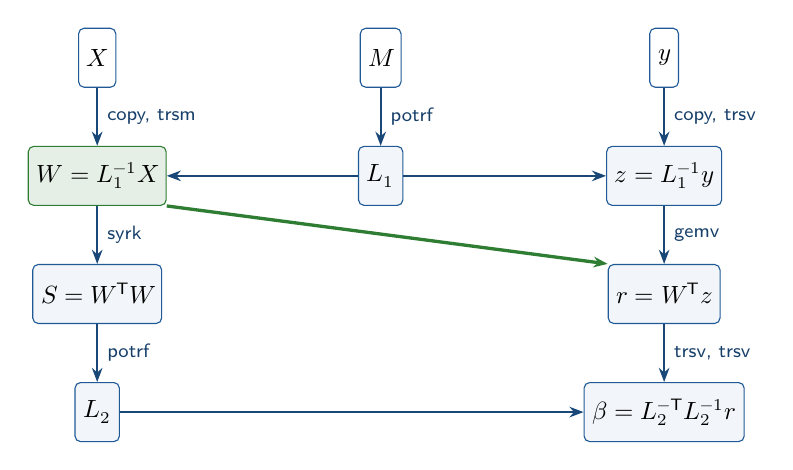
\begin{tikzpicture}[font=\sffamily\small,
  v/.style={draw=accent,fill=accent!6,rounded corners=2pt,minimum height=0.75cm,
    align=center,inner sep=3pt},
  inp/.style={v,fill=white},
  k/.style={font=\sffamily\scriptsize,text=accent!70!black},
  arr/.style={-{Stealth[length=1.8mm]},draw=accent!80!black,semithick}]
  \node[inp] (X) at (0,0) {\(X\)};
  \node[inp] (M) at (3.6,0) {\(M\)};
  \node[inp] (y) at (7.2,0) {\(y\)};
  \node[v,fill=oinf!12,draw=oinf] (W) at (0,-1.5) {\(W = L_1\inv X\)};
  \node[v] (L1) at (3.6,-1.5) {\(L_1\)};
  \node[v] (z) at (7.2,-1.5) {\(z = L_1\inv y\)};
  \node[v] (S) at (0,-3) {\(S = W\T W\)};
  \node[v] (r) at (7.2,-3) {\(r = W\T z\)};
  \node[v] (L2) at (0,-4.5) {\(L_2\)};
  \node[v] (b) at (7.2,-4.5) {\(\beta = L_2\invT L_2\inv r\)};
  \draw[arr] (X) -- node[k,right] {copy, trsm} (W);
  \draw[arr] (M) -- node[k,right] {potrf} (L1);
  \draw[arr] (y) -- node[k,right] {copy, trsv} (z);
  \draw[arr] (L1) -- (W);
  \draw[arr] (L1) -- (z);
  \draw[arr] (W) -- node[k,right] {syrk} (S);
  \draw[arr] (S) -- node[k,right] {potrf} (L2);
  \draw[arr,draw=oinf,very thick] (W.south east) -- (r.north west);
  \draw[arr] (z) -- node[k,right] {gemv} (r);
  \draw[arr] (r) -- node[k,right] {trsv, trsv} (b);
  \draw[arr] (L2) -- (b);
\end{tikzpicture}
\caption{Values and dependences of the selected kernels. \(W\) (green) has
two uses; \(L_1\) has two uses. Each value is computed once.}
\label{fig:gls-dag}
\end{figure}

\begin{theory}[ (\FGs{4.5}, \FGs{3.3})]
Kernel selection is instruction selection with BLAS and LAPACK as the
instruction set: leaves are operands, kernels are tiles that cover an
interval of the product, and the dynamic program picks the cheapest tiling,
as in tree tiling with dynamic programming,
\FG{4.5}{Instruction selection: tree/DAG tiling, SelectionDAG vs
GlobalISel}. The interval structure is that of the matrix chain problem
(generalized to solves and transposes by Barthels et al.~\cite{gmc}). The
pass replaces one dialect by another in a single step and keeps the
structure needed later (DPS, flags), which is \emph{progressive lowering},
\FG{3.3}{Progressive lowering and the dialect conversion framework}.
It does \emph{not} use MLIR's dialect conversion framework: it is a custom
C++ traversal (\cref{sec:kernels-select}).
\end{theory}

\begin{limit}
The selected sequence equals the formula \emph{over the real numbers}. In
floating point it is a different computation with different rounding:
\(W\T W\) is not bitwise \((X\T M\inv) X\), and its accuracy depends on the
condition number of \(W\) squared. \Cref{sec:gls-numbers} shows a
difference in the last bit; \cref{sec:kernels-fp} shows a case where the
two differ completely.
\end{limit}

% ---------------------------------------------------------------------------
\section{From values to memory: bufferization, workspace and \texttt{info}}
\label{sec:gls-storage}

\begin{steps}
\item[Input] kernels on tensors in DPS; read-only arguments marked \code{ulm_lam.in}.
\item[Representation] after bufferization: kernels on \code{memref}s, with no results.
\item[Rule] One-Shot Bufferize writes a kernel's result into the buffer of its \code{outs} operand unless that buffer is read-only or still read later; then it copies first.
\item[Output] \texttt{6-bufferized.mlir}: three copies, one workspace, an \code{info} result.
\item[Theory] \FG{10.3}{Bufferization and destination-passing style}; \FG{2.7}{Value semantics vs reference/memory semantics in IRs}.
\end{steps}

The core of the bufferized function (the workspace protocol at its start
and the \code{scf.if} nesting of the \code{info} checks are left out; see
\cref{sec:storage-workspace} for both):

\begin{lstlisting}
%view = memref.view %25[%c0][%arg0, %arg0] : memref<?xi8> to memref<?x?xf64>
memref.copy %arg3, %view : memref<?x?xf64> to memref<?x?xf64>          // copy of M
%info = ulm_lamk.potrf uplo(lower) outs(%view : memref<?x?xf64>)        // L1 in the copy
...                                                                     // if info == 0:
%view_1 = memref.view %25[%4][%arg1, %arg1] : memref<?xi8> to memref<?x?xf64>
%view_2 = memref.view %25[%9][%arg0, %arg1] : memref<?xi8> to memref<?x?xf64>
ulm_lamk.gecopy trans(trans) ins(%arg2 : memref<?x?xf64>) outs(%view_2 : memref<?x?xf64>)
ulm_lamk.trsm side(left) uplo(lower) trans(none) diag(non_unit) alpha(%cst)
    ins(%view : memref<?x?xf64>) outs(%view_2 : memref<?x?xf64>)       // W
ulm_lamk.syrk uplo(lower) trans(trans) alpha(%cst) beta(%cst_0)
    ins(%view_2 : memref<?x?xf64>) outs(%view_1 : memref<?x?xf64>)     // S
%info_3 = ulm_lamk.potrf uplo(lower) outs(%view_1 : memref<?x?xf64>)   // L2
...                                                                     // if info_3 == 0:
%view_4 = memref.view %25[%13][%arg0] : memref<?xi8> to memref<?x1xf64>
memref.copy %arg4, %view_4 : memref<?x1xf64> to memref<?x1xf64>        // copy of y
ulm_lamk.trsv ... ins(%view : memref<?x?xf64>) outs(%view_4 : memref<?x1xf64>)        // z
ulm_lamk.gemv trans(trans) ... ins(%view_2, %view_4 : ...) outs(%arg5 : memref<?x1xf64>)
ulm_lamk.trsv uplo(lower) trans(none) ... ins(%view_1 : ...) outs(%arg5 : memref<?x1xf64>)
ulm_lamk.trsv uplo(lower) trans(trans) ... ins(%view_1 : ...) outs(%arg5 : memref<?x1xf64>)
\end{lstlisting}

\paragraph{Why three copies} \code{potrf} overwrites its matrix, \code{trsm}
and \code{trsv} their right-hand sides. \(M\), \(X\) and \(y\) are
\code{ulm_lam.in}, so \code{ulm-lam-results-to-out-params} gave them
\code{bufferization.writable = false}
(\srcref{lib/UlmLamResultsToOutParams.cpp}{344}{368}), and One-Shot
Bufferize must not write into them: it copies \(M\) and \(y\). For \(X\)
the copy was already in the IR (\code{gecopy}, a transposing copy that
\code{trsm} then overwrites), so no further copy is needed. With
\code{InOut(...)} parameters the caller allows overwriting;
\code{examples/gls/check.sh} verifies that \code{potrf} then works on the
caller's \(M\) and only \(X\) is copied.

\paragraph{One value, two uses, one buffer} \(W\) lives in \code{\%view_2},
written once by \code{trsm} and read by \code{syrk} and \code{gemv}. SSA
use counts are not copies: a value with two uses needs a second buffer only
if one use would overwrite it while the other still reads it.

\paragraph{The result} \(\beta\) is computed directly in the caller's
output buffer \code{\%arg5}: \code{gemv} writes it, the two \code{trsv}
update it in place.

\paragraph{The workspace} All temporaries are views of one byte buffer
\code{\%25} at offsets computed from \(n\) and \(m\), each rounded up to 64
bytes (\cref{fig:workspace}). The caller can pass that buffer, query its size
first (LAPACK's \code{lwork} convention), or let the function allocate it.

\paragraph{\code{info}} Each factorization is a numbered check. If
\code{potrf} reports failure, the rest of the block does not run and the
function returns the check's number. In C++ this is the return value of
\code{gls}; in Julia, an \code{InfoError}.

\begin{theory}[ (\FGs{10.3}, \FGs{2.7}, \FGs{1.4})]
Tensors have value semantics, memrefs reference semantics,
\FG{2.7}{Value semantics vs reference/memory semantics in IRs}.
Bufferization chooses, for every DPS result, between reusing the
destination's buffer and copying, \FG{10.3}{Bufferization and
destination-passing style}. The in-place condition (no other live reader of
the old value, and the buffer may be written) is a uniqueness condition, as
\FG{1.4}{Uniqueness types vs linear types} explains; here it is decided by
an analysis, not by a type system. \Cref{ch:storage} goes into detail.
\end{theory}

% ---------------------------------------------------------------------------
\section{The kernel sequence in C++}
\label{sec:gls-kernels}

\code{convert-ulm-lamk-to-ulmblas} lowers the memref program to the EmitC
dialect, and \code{mlir-translate --mlir-to-cpp} prints C++. With the
Julia backend the calls go to CBLAS (the C interface to BLAS) and LAPACK
through Julia's libblastrampoline, which forwards them to OpenBLAS here. The
calls of \texttt{7-gls.cpp}, in order (\code{v1} \(=n\), \code{v2} \(=m\),
\code{v3} \(=X\T\) row-major, \code{v4} \(=M\), \code{v5} \(=y\),
\code{v6} \(=\beta\)):

\begin{lstlisting}[style=cpp]
ulm_lam_copy(v31, v4, v32);                                          // M -> workspace
int64_t v33 = ulm_lam_cblas::potrf<std::ptrdiff_t>(true, v1, v31, v1, 1);
ulm_lam_gecopy(v1, v2, v3, 1, v1, v41, v2, 1);                       // X (transposing copy)
(void)ulm_lam_cblas::trtrs<std::ptrdiff_t>(
    true, false, false, false, v1, v2, v31, v1, 1, v41, v2, 1);      // W = L1^-1 X
ulm_lam_cblas::sylrk<std::ptrdiff_t>(v2, v1, v9, v41, 1, v2,
                                     v10, v39, v2, 1);               // S = W^T W (lower)
int64_t v42 = ulm_lam_cblas::potrf<std::ptrdiff_t>(true, v2, v39, v2, 1);
ulm_lam_copy(v45, v5, v46);                                          // y -> workspace
ulm_lam_cblas::trlsv<std::ptrdiff_t>(v1, false, v31, v1, 1, v45, 1);  // z = L1^-1 y
ulm_lam_cblas::gemv<std::ptrdiff_t>(v2, v1, v9, v41, 1, v2,
                                    v45, 1, v10, v6, 1);             // beta = W^T z
ulm_lam_cblas::trlsv<std::ptrdiff_t>(v2, false, v39, v2, 1, v6, 1);   // beta = L2^-1 beta
ulm_lam_cblas::trusv<std::ptrdiff_t>(v2, false, v39, 1, v2, v6, 1);   // beta = L2^-T beta
\end{lstlisting}

Two details show what lowering does with the remaining structure. The
transposition flags are gone: a transposed operand is the same pointer with
swapped strides (\code{v39, 1, v2} versus \code{v39, v2, 1}), so
\(L_2\T\) is passed as an \emph{upper} triangular matrix to
\code{trusv}. And the matrix properties are gone entirely; what is left of
them is the choice of routines and their \code{uplo} arguments.

\begin{center}\small
\begin{tabularx}{\linewidth}{@{}lllL@{}}
\toprule
\textbf{Kernel} & \textbf{Library} & \textbf{Flops} & \textbf{Computes} \\
\midrule
\code{potrf} & LAPACK & \(n^3/3\) & \(M = L_1 L_1\T\), in a copy of \(M\) \\
\code{trsm} (\code{trtrs}) & BLAS 3 & \(n^2 m\) & \(W = L_1\inv X\), in a copy of \(X\) \\
\code{syrk} & BLAS 3 & \(n m^2\) & \(S = W\T W\), lower triangle \\
\code{potrf} & LAPACK & \(m^3/3\) & \(S = L_2 L_2\T\), in place \\
\code{trsv} & BLAS 2 & \(n^2\) & \(z = L_1\inv y\), in a copy of \(y\) \\
\code{gemv} & BLAS 2 & \(2nm\) & \(\beta \leftarrow W\T z\) \\
\code{trsv}, \code{trsv} & BLAS 2 & \(2m^2\) & \(\beta \leftarrow L_2\invT L_2\inv \beta\) \\
\bottomrule
\end{tabularx}
\end{center}

% ---------------------------------------------------------------------------
\section{A numerical example}
\label{sec:gls-numbers}

Small inputs make every step checkable by hand. Take \(n=4\), \(m=2\),
\[
X=\begin{pmatrix}1&0\\1&1\\1&2\\1&3\end{pmatrix},\quad
M=\begin{pmatrix}4&2&0&0\\2&5&2&0\\0&2&5&2\\0&0&2&5\end{pmatrix},\quad
y=\begin{pmatrix}1\\2\\4\\4\end{pmatrix}.
\]
\(M\) is SPD (eigenvalues between 1.58 and 8.13) with Cholesky factor
\(L_1\) = 2 on the diagonal and 1 below it, so every step up to \(S\) is
exact in binary floating point:
\[
W = L_1\inv X = \begin{pmatrix}1/2&0\\1/4&1/2\\3/8&3/4\\5/16&9/8\end{pmatrix},\quad
S = W\T W = \begin{pmatrix}141/256 & 97/128\\ 97/128 & 133/64\end{pmatrix},\quad
X\T M\inv y = \begin{pmatrix}363/256\\375/128\end{pmatrix}.
\]

\paragraph{Expected} In exact rational arithmetic,
\[
  \beta = \Bigl(\frac{93}{73},\ \frac{69}{73}\Bigr) = (1.273972602739726\ldots,\ 0.945205479452054\ldots).
\]

\paragraph{Obtained} \code{examples/gls.jl} prints:

\begin{textout}
==== exact β (rational): Rational{BigInt}[93//73, 69//73]
==== exact β (Float64):  [1.273972602739726, 0.9452054794520548]
==== ulm.lam β: [1.2739726027397262, 0.9452054794520546]
==== Julia expert  (X'*(M\X)) \ (X'*(M\y)): [1.2739726027397262, 0.9452054794520547]
==== Julia formula inv(X'*inv(M)*X)*X'*inv(M)*y: [1.2739726027397262, 0.9452054794520547]
==== max abs error vs exact: 2.220446049250313e-16
\end{textout}

ulm.lam's result differs from the correctly rounded \(\beta\) by one unit
in the last place in each component, and from Julia's two evaluations in the
second component by one unit. All three are correct to working accuracy;
they differ because they round differently, not because one is wrong.

\paragraph{Failing and rejected inputs} The same program with inputs that
violate its assumptions (all from \code{outputs/gls.out}):

\begin{center}\small
\begin{tabularx}{\linewidth}{@{}P{4.6cm}P{5.3cm}L@{}}
\toprule
\textbf{Input} & \textbf{Result} & \textbf{Origin of the check} \\
\midrule
\(M_{33} = -1\): symmetric, indefinite & \code{InfoError: gls: info 1: Cholesky factorisation of v4: not positive definite} & \Orun: \code{potrf} of \(M\) \\
\(X\) with two equal columns, declared \code{full_rank} & \code{InfoError: gls: info 2: Cholesky factorisation of a computed matrix: not positive definite} & \Orun: \code{potrf} of \(S\) \\
\(y\) of length 3 & \code{LamError: gls: y: size :n = 3, but 4 from an earlier argument} & \Orun: the Julia runtime compares sizes before the call \\
\(M_{12} = 100\) (Julia's upper triangle), declared \code{spd} & \code{InfoError: ... info 1 ...} & \Orun, by luck: \code{potrf} reads the triangle that was changed \\
\(M_{21} = 100\) (Julia's lower triangle), declared \code{spd} & \(\beta\) of \code{Symmetric(M, :U)}; no error & \Onone: symmetry is never checked, one triangle is ignored \\
\code{Mat(:n,:m) * Mat(:n,:m)} in a \code{@lam} body & \code{LamError: product of nxm and nxm: m columns but n rows} & at trace time, by the frontend (\cref{ch:shapes}) \\
\bottomrule
\end{tabularx}
\end{center}

Two remarks. The messages name \code{v4}, the fourth C parameter, where
\code{@code_lam} says \code{M}: the description comes from the C++
interface comment. And the rank-deficient \(X\) is caught only because
\(S\) became exactly singular here. A nearly rank-deficient \(X\) can pass
the factorization and give an inaccurate \(\beta\), or fail although \(X\)
has full rank (\cref{sec:kernels-fp}).

% ---------------------------------------------------------------------------
\section{The chapter in one table}
\label{sec:gls-summary}

\begin{center}\small
\begin{tabularx}{\linewidth}{@{}P{3.1cm}P{4.6cm}P{3.3cm}L@{}}
\toprule
\textbf{Step} & \textbf{MLIR mechanism} & \textbf{Theory} & \textbf{FG} \\
\midrule
tracing & text emitted by overloaded Julia operators & tracing eDSL & \FGs{3.7} \\
facts on matrices & builtin tensor type with an attribute in its encoding & refinement types & \FGs{1.7} \\
normal form & \code{OpRewritePattern}s, greedy driver & rewriting, termination & \FGs{3.4}, \FGs{3.5} \\
\(X\T M\inv X\) is SPD & \code{InferTypeOpInterface} per op & type inference; abstract interpretation & \FGs{1.10}, \FGs{5.2} \\
kernel selection & custom pass, DP over leaves & instruction selection & \FGs{4.5}, \FGs{3.3} \\
copies, in place & DPS ops, One-Shot Bufferize & value vs reference semantics; uniqueness & \FGs{10.3}, \FGs{2.7}, \FGs{1.4} \\
failed factorization & \code{info} results, \code{scf.if} & run-time check & --- \\
C++ & dialect conversion to EmitC & lowering, legalization & \FGs{3.3}, \FGs{4.6} \\
\bottomrule
\end{tabularx}
\end{center}

% ch2-infrastructure.tex
\chapter{MLIR Provides the Infrastructure, ulm.lam Provides the Meaning}
\label{ch:infra}

\begin{answer}
MLIR~\cite{mlir} has an open, extensible type system. A dialect defines its own types,
attributes and operations, and states the rules that they must satisfy;
MLIR runs those rules at defined points and rejects IR that breaks them. MLIR
does not come with any particular type \emph{discipline}: not linear types,
not dependent types, not refinement types, not an effect system. Each of
those needs a semantics and an enforcement mechanism that someone has to
design and implement. In short: \emph{MLIR provides the infrastructure for
representing domain-specific types and enforcing rules about operations.
The meaning of those types, and the strength of the guarantees they provide,
comes from the dialect and its implementation.}
\end{answer}

The Field Guide describes the infrastructure side in \FG{3.1}{Dialects and
extensible operation sets} and \FG{3.2}{Traits and interfaces}, and the
type disciplines in \FGch{1}{Types as Static Resource Reasoning}. This
chapter shows, with ulm.lam, which of the two you are looking at in each
case.

% ---------------------------------------------------------------------------
\section{Who provides what}
\label{sec:infra-who}

\begin{table}[h]
\centering\small
\begin{tabularx}{\linewidth}{@{}P{2.4cm}LL@{}}
\toprule
\textbf{Concern} & \textbf{MLIR provides} & \textbf{ulm.lam implements} \\
\midrule
types & builtin \code{tensor} and \code{memref} with an \emph{encoding}
  slot; ODS (Operation Definition Specification, in TableGen) for new
  types and attributes &
  no new type; one attribute, \code{#ulm_lam.props<...>}, used as tensor
  encoding \\
operations & ODS: operands, results, type constraints, assembly format &
  \code{ulm_lam}: 7 ops (\code{mul}, \code{add}, \code{scale},
  \code{transpose}, \code{inverse}, \code{identity}, \code{assume});
  \code{ulm_lamk}: 17 kernel ops and \code{call} \\
verification & hooks (\code{verify()}, \code{verifyEncoding}), generated
  operand checks, \code{InferTypeOpInterface}'s result check; run after
  parsing and (by default) after each pass &
  the rules: inner dimensions, squareness, contradictory properties, DPS
  result types \\
inference & \code{InferTypeOpInterface} and its compatibility hook
  \code{isCompatibleReturnTypes} & the property rules (\code{mulProperties},
  \ldots) and what ``compatible'' means \\
effects & \code{MemoryEffectOpInterface}, the \code{Pure} trait; generic
  passes (CSE, DCE (dead code elimination), LICM (loop-invariant code
  motion)) that consult them & which ops are pure; which
  operands a kernel reads and writes \\
rewriting & pattern classes, the greedy driver, the dialect conversion
  framework & the normal form, kernel selection, the lowering to EmitC \\
memory & One-Shot Bufferize; \code{DstBufferizableOpInterfaceExternalModel}
  for DPS ops & DPS kernel ops and their bufferization models; the
  workspace and \code{info} passes \\
\bottomrule
\end{tabularx}
\caption{The division of labor between MLIR and ulm.lam.}
\label{tab:infra-who}
\end{table}

Read the table column by column. Everything on the left is generic and
knows nothing about matrices. Everything on the right is a decision of
ulm.lam. When this text says that ``the compiler knows that \(S\) is SPD'',
the knowledge is in the right column: MLIR stores the attribute, calls the
inference hook and runs the verifier, but the meaning of \code{spd} and the
rule that derives it are ulm.lam's C++.

% ---------------------------------------------------------------------------
\section{A property set as a tensor encoding}
\label{sec:infra-props}

\begin{steps}
\item[Input] a type written as \code{tensor<?x?xf64, #ulm_lam.props<spd>>}.
\item[Representation] a builtin \code{RankedTensorType} whose encoding is a \code{PropertiesAttr}, a 32-bit set of named facts.
\item[Rule] \code{verifyEncoding}, called by MLIR whenever such a type is built or parsed.
\item[Output] the type, or a diagnostic.
\item[Theory] a refinement of the base type by a predicate, \FG{1.7}{Refinement types}.
\end{steps}

The declaration (\srcref{include/ulm_lam/UlmLamAttrs.td}{37}{77}, cases
shortened):

\begin{lstlisting}[style=td]
def UlmLam_PropSquare     : I32BitEnumAttrCaseBit<"square",       0>;
def UlmLam_PropSymmetric  : I32BitEnumAttrCaseBit<"symmetric",    1>;
def UlmLam_PropSPSD       : I32BitEnumAttrCaseBit<"spsd",         2>;
def UlmLam_PropSPD        : I32BitEnumAttrCaseBit<"spd",          3>;
...
def UlmLam_PropFullRank   : I32BitEnumAttrCaseBit<"full_rank",   12>;
def UlmLam_PropLowerStored: I32BitEnumAttrCaseBit<"lower_stored",13>;
def UlmLam_PropUpperStored: I32BitEnumAttrCaseBit<"upper_stored",14>;
def UlmLam_PropDiagonal   : I32BitEnumAttrCaseGroup<"diagonal",
                              [UlmLam_PropLowerTri, UlmLam_PropUpperTri]>;
...
// Used as a builtin tensor encoding:  tensor<?x?xf64, #ulm_lam.props<spd>>
def UlmLam_PropsAttr : EnumAttr<UlmLam_Dialect, UlmLam_Properties, "props",
    [DeclareAttrInterfaceMethods<VerifiableTensorEncoding>]> {
  let assemblyFormat = "`<` $value `>`";
  ...
}
\end{lstlisting}

Two MLIR mechanisms carry it: \code{EnumAttr} over an \code{I32BitEnumAttr}
generates the attribute class, its parser and printer; the interface
\code{VerifiableTensorEncoding} makes MLIR call a verifier when a tensor
type with this encoding is created. The verifier is ulm.lam's
(\srcref{lib/UlmLamDialect.cpp}{145}{167}):

\begin{lstlisting}[style=cpp]
LogicalResult PropertiesAttr::verifyEncoding(ArrayRef<int64_t> shape, Type,
    function_ref<InFlightDiagnostic()> emitError) const
{
    P p = closure(getValue(), shape);
    if (shape.size() != 2)
        return emitError() << "#ulm_lam.props needs a rank-2 tensor";
    if (has(p, P::zero) && has(p, P::full_rank))
        return emitError() << "#ulm_lam.props: zero contradicts full rank";
    ...
    if (has(p, P::square) && !ShapedType::isDynamic(shape[0]) &&
        !ShapedType::isDynamic(shape[1]) && shape[0] != shape[1])
        return emitError() << "#ulm_lam.props: square property on a "
                           << shape[0] << "x" << shape[1] << " tensor";
    return success();
}
\end{lstlisting}

It first closes the set under implication (so \code{spd} brings
\code{square}), then checks the closure against itself and against the
static shape. Two rejected types (\code{outputs/verify.out}):

\begin{textout}
### v3-square-props.mlir
v3-square-props.mlir:1:53: error: #ulm_lam.props: square property on a 3x4 tensor
func.func @f(%a: tensor<3x4xf64, #ulm_lam.props<spd>>) {
### v4-zero-fullrank.mlir
v4-zero-fullrank.mlir:1:68: error: #ulm_lam.props: zero contradicts full rank
func.func @f(%a: tensor<?x?xf64, #ulm_lam.props<zero, non_singular>>) {
\end{textout}

\code{spd} on a \(3\times 4\) tensor is rejected because SPD implies square;
\code{zero} with \code{non_singular} because non-singular implies full rank.
Both are contradictions \emph{between the facts and the shape}, decided
without looking at any data. \code{tensor<4x4xf64, #ulm_lam.props<spd>>} is
accepted for every \(4\times 4\) matrix, SPD or not: a type cannot be wrong
about entries it never sees.

% ---------------------------------------------------------------------------
\section{Operation verifiers: structural rules}
\label{sec:infra-verify}

Each op class may define \code{verify()}. MLIR calls it after parsing and,
with the default pass-manager settings, after every pass. For
\code{ulm_lam.mul} (\srcref{lib/UlmLamDialect.cpp}{514}{526}):

\begin{lstlisting}[style=cpp]
LogicalResult MulOp::verify()
{
    if (getFactors().size() < 2)
        return emitOpError("needs at least two factors");
    for (unsigned i = 0; i + 1 < getFactors().size(); ++i) {
        Type a = getFactors()[i].getType(), b = getFactors()[i + 1].getType();
        if (!dimsCompatible(cols(a), rows(b)))
            return emitOpError("factor ") << i << " has " << cols(a)
                   << " columns but factor " << i + 1 << " has " << rows(b) << " rows";
    }
    return success();
}
\end{lstlisting}

\code{dimsCompatible(a, b)} is true if either is dynamic or both are equal.
Accepted and rejected (\code{outputs/verify.out}):

\begin{textout}
### v1-mul-static.mlir
v1-mul-static.mlir:2:8: error: 'ulm_lam.mul' op factor 0 has 4 columns but factor 1 has 5 rows
### v2-mul-dynamic.mlir
accepted
### v5-inverse-nonsquare.mlir
v5-inverse-nonsquare.mlir:2:8: error: 'ulm_lam.inverse' op operand is not square
### v9-gemm.mlir
v9-gemm.mlir:3:8: error: 'ulm_lamk.gemm' op shapes of op(A), op(B) and C do not match
### v10-gemm-dps.mlir
v10-gemm-dps.mlir:3:8: error: 'ulm_lamk.gemm' op result 0 must have the type of its init
\end{textout}

\code{v2} multiplies two \code{tensor<?x?xf64>}: the verifier cannot know
whether the inner sizes agree, so it accepts. \Cref{ch:shapes} shows where
dynamic sizes \emph{are} checked. \code{v10} violates a DPS rule: a kernel's
tensor result must have the type of the operand it overwrites
(\code{verifyDps}, \srcref{lib/UlmLamDialect.cpp}{826}{845}).

\begin{limit}
An operation verifier checks the IR, not the data. It sees types,
attributes and the structure of the program, and it runs at compile time.
It cannot tell whether the \(4\times 4\) array that a caller passes is SPD.
In ulm.lam that question is answered only by \code{potrf} at run time, and
only for the matrices that get factorized.
\end{limit}

% ---------------------------------------------------------------------------
\section{Result types must be justified}
\label{sec:infra-compat}

\begin{steps}
\item[Input] an op whose result type is written out, possibly with properties.
\item[Representation] \code{ulm_lam} ops implement \code{InferTypeOpInterface}.
\item[Rule] MLIR's generated verifier infers the result type from the operands and calls \code{isCompatibleReturnTypes(inferred, declared)}; ulm.lam defines compatible as ``same shape up to \code{?}, same element type, and every declared property is implied by the inferred ones''.
\item[Output] a declared type may be weaker than the inferred one, never stronger.
\item[Theory] subtyping by implication, \FG{1.7}{Refinement types}; checking against an annotation, \FG{1.10}{Type inference beyond Hindley–Milner: bidirectional and constraint-based}.
\end{steps}

The compatibility relation (\srcref{lib/UlmLamDialect.cpp}{359}{380}):

\begin{lstlisting}[style=cpp]
/// Shapes compatible, element types equal, properties of `actual` implied
/// by `inferred`.
bool ulmLamCompatible(TypeRange inferred, TypeRange actual)
{
    ...
        P have = closure(propertiesOf(it), it.getShape());
        if (!has(have, propertiesOf(at)))
            return false;
    ...
}
\end{lstlisting}

The test is the pair \code{v6} and \code{v7}: the same Gram product
\(A\T A\) of a \(4\times 3\) matrix, with the result declared \code{spd}.
Without \code{full_rank} on \(A\), only SPSD can be inferred, and the
verifier rejects the claim:

\begin{textout}
### v6-overclaim.mlir
v6-overclaim.mlir:3:8: error: 'ulm_lam.mul' op inferred type(s) 'tensor<3x3xf64, #ulm_lam.props<spsd>>' are incompatible with return type(s) of operation 'tensor<3x3xf64, #ulm_lam.props<spd>>'
v6-overclaim.mlir:3:8: error: 'ulm_lam.mul' op failed to infer returned types
### v7-overclaim-ok.mlir
accepted
\end{textout}

With \code{full_rank} on \(A\) (\code{v7}), SPD is inferable and the same
declaration is accepted. So inside a function, a property on a result type
is not an assumption: it is a claim that the verifier checks against the
inference rules. The only way to state more than inference derives is the
dedicated op \code{ulm_lam.assume}, which has no inference hook and is
accepted with any properties (\code{v8} in \code{outputs/verify.out}).
\Cref{sec:facts-declared} discusses it.

\begin{theory}[ (\FGs{1.7}, \FGs{1.10})]
In a refinement type system, a value of type \(\{v{:}B \mid p\}\) may be
used where \(\{v{:}B \mid q\}\) is expected if \(p \Rightarrow q\). Here
\(B\) is the tensor type, \(p\) the inferred property set and \(q\) the
declared one, and \(p \Rightarrow q\) is decided by closing \(p\) under the
implication rules and testing bit-set containment, not by an SMT
(satisfiability modulo theories) solver: with fifteen atoms and a fixed set
of Horn-like implications the check is a few bit operations. Comparing a
synthesized type against a written one is the \emph{checking} direction of
bidirectional typing.
\end{theory}

% ---------------------------------------------------------------------------
\section{Operation traits are not matrix properties}
\label{sec:infra-traits}

Both are called ``properties'' in casual speech, and both are written in
ODS. They live in different worlds.

\begin{center}\small
\begin{tabularx}{\linewidth}{@{}P{3.3cm}LL@{}}
\toprule
 & \textbf{Op traits and interfaces} & \textbf{Matrix properties} \\
\midrule
example & \code{Pure}, \code{Commutative}, \code{DestinationStyleOpInterface} & \code{spd}, \code{lower_tri}, \code{full_rank} \\
describes & an \emph{operation class} (all \code{ulm_lam.mul} ops) & a \emph{value} (this matrix) \\
where & the op's C++ class, via ODS & the value's type (encoding) \\
read by & generic MLIR passes: CSE, DCE, LICM, canonicalizer, bufferization & only ulm.lam's own rules and passes \\
MLIR understands it & yes: that is its purpose & no: an opaque attribute \\
\bottomrule
\end{tabularx}
\end{center}

\code{ulm_lam.add} has the trait \code{Commutative}
(\srcref{include/ulm_lam/UlmLamOps.td}{63}{71}); \code{ulm_lam.mul} does
not, because matrix products do not commute. The trait states a fact about
the \emph{operation} that a generic canonicalizer may use (to sort
operands). A matrix being SPD states a fact about the \emph{operand}, and no
upstream pass will ever read it.

\begin{limit}
MLIR operation traits are not mathematical matrix properties. The trait
\code{Pure} on \code{ulm_lam.inverse} says that the operation has no memory
effects and may be executed speculatively; it says nothing about whether the
operand is invertible. \Cref{sec:effects-speculation} shows what follows
from that difference.
\end{limit}

% ---------------------------------------------------------------------------
\section{What is present, and what is related by analogy}
\label{sec:infra-analogy}

\begin{table}[t]
\centering\small
\begin{tabularx}{\linewidth}{@{}P{3.2cm}LP{2.4cm}@{}}
\toprule
\textbf{Discipline (FG)} & \textbf{In ulm.lam} & \textbf{Status} \\
\midrule
refinement types (\FGs{1.7}) & property sets on tensor types; results
  checked by implication; parameters and \code{assume} trusted &
  \textbf{present}, with a finite predicate language \\
type inference (\FGs{1.10}) & synthesis of result types per op, one pass
  in program order & \textbf{present} \\
indexed / dependent types (\FGs{1.8}) & static shapes checked; run-time
  sizes named in the Julia frontend and in \code{ulm_lam.dims}; no
  type-level terms & \textbf{analogy} (\cref{ch:shapes}) \\
effect systems (\FGs{1.6}) & per-op memory effects, used by generic
  passes; no effects in function types, no effect polymorphism &
  \textbf{partly}: effect annotations, not an effect type system \\
linear / affine types (\FGs{1.2}, \FGs{1.3}) & none: SSA values may be
  used any number of times & \textbf{absent} (\cref{ch:values}) \\
uniqueness (\FGs{1.4}) & the in-place condition of bufferization, decided
  by an analysis & \textbf{analogy} (\cref{ch:storage}) \\
region types (\FGs{1.5}) & none; MLIR regions are nested code, the
  workspace is one arena per call & \textbf{absent}; analogy only \\
typestate (\FGs{1.9}) & ``factorized'' is tracked by a memo table in
  kernel selection, not in types & \textbf{absent} \\
\bottomrule
\end{tabularx}
\caption{Type disciplines of FG Chapter 1 and their status in ulm.lam.}
\label{tab:infra-status}
\end{table}

\Cref{tab:infra-status} is the short answer to ``which theoretical type
systems does ulm.lam have?''. Three entries need a remark.

\paragraph{Declared but not implemented} The ODS of \code{ulm_lam.assume}
has a unit attribute \code{checked}, documented as ``verified at run time
(e.g.\ symmetry test, or success of the Cholesky factorisation for spd)''
(\srcref{include/ulm_lam/UlmLamOps.td}{135}{154}). At commit
\texttt{\shortcommit} neither frontend sets it and no pass generates a
check from it; the only code that reads it is a normalization pattern that
leaves checked assumptions alone
(\srcref{lib/UlmLamPasses.cpp}{79}{99}). Likewise, the pass description in
\srcfile{include/ulm_lam/UlmLamPasses.td} lists kernel-selection strategies
\code{search} and \code{egraph}, a \code{cost-model} option and a pass
\code{convert-ulm-lamk-to-linalg}; that file is documentation (the passes
are registered by hand in C++), and the implemented pass rejects every
strategy but \code{gmc} (\srcref{lib/UlmLamPasses.cpp}{2295}{2305}).

\paragraph{Interfaces that nothing calls} \code{ulm_lam} and
\code{ulm_lamk} ops implement two interfaces of ulm.lam's own,
\code{PropertyInferenceOpInterface} and \code{KernelCostOpInterface}
(\srcref{include/ulm_lam/UlmLamInterfaces.td}{11}{48}). No pass at this
commit calls them: inference goes through MLIR's
\code{InferTypeOpInterface}, and kernel selection computes flop counts
inline (\cref{sec:orders-cost}). They are the extension points of a design,
not mechanisms of the current compiler.

\paragraph{Effects are partly present} MLIR's effect interface is a real
effect annotation per op, and generic passes use it soundly
(\cref{ch:values}). What the Field Guide calls an effect \emph{system},
effects in function types that compose by union and that a type checker
verifies, does not exist in MLIR or in ulm.lam.

% ch3-facts.tex
\chapter{Assumed, Verified, Inferred, Checked: Where Facts Come From}
\label{ch:facts}

\begin{answer}
ulm.lam proves nothing about the entries of a matrix. Facts enter in two
places only, the parameter types and \code{assume}, and are trusted there.
Inference rules derive new facts from them; these are theorems about real
matrices, valid if the declarations are. Verifiers check that the IR is
consistent with the rules, never with the data. At run time the Julia (or
Python) runtime checks the array sizes, and each factorization checks the
one fact it depends on: \code{potrf} detects a matrix that is not positive
definite in floating point, \code{getrf} an exactly singular one. Symmetry
of an input, full column rank and conditioning are not checked.
\end{answer}

% ---------------------------------------------------------------------------
\section{The facts and how they imply each other}
\label{sec:facts-lattice}

A property set is a conjunction of atoms. Its meaning is fixed by one C++
function, \code{closure} (\srcref{lib/UlmLamDialect.cpp}{97}{123}), which
adds everything that the given atoms imply (\cref{fig:implications}).

\begin{figure}[h]
\centering
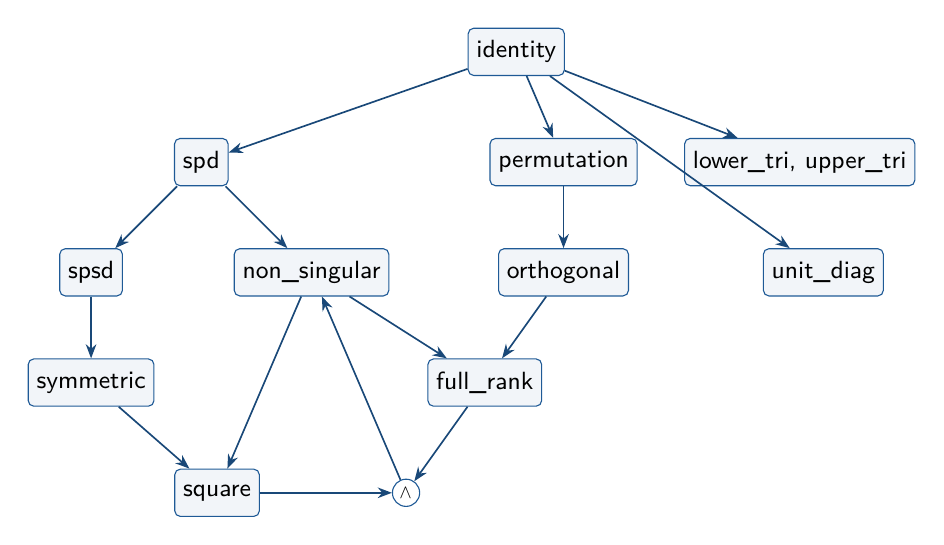
\begin{tikzpicture}[font=\sffamily\small,
  p/.style={draw=accent,fill=accent!6,rounded corners=2pt,inner sep=3pt,minimum height=0.6cm},
  c/.style={draw=accent,circle,fill=white,inner sep=1.2pt,font=\sffamily\scriptsize},
  arr/.style={-{Stealth[length=1.8mm]},draw=accent!80!black,semithick}]
  \node[p] (id) at (0,0) {identity};
  \node[p] (spd) at (-4.0,-1.4) {spd};
  \node[p] (perm) at (0.6,-1.4) {permutation};
  \node[p] (tri) at (3.6,-1.4) {lower\_tri, upper\_tri};
  \node[p] (ud) at (3.9,-2.8) {unit\_diag};
  \node[p] (spsd) at (-5.4,-2.8) {spsd};
  \node[p] (ns) at (-2.6,-2.8) {non\_singular};
  \node[p] (orth) at (0.6,-2.8) {orthogonal};
  \node[p] (sym) at (-5.4,-4.2) {symmetric};
  \node[p] (fr) at (-0.4,-4.2) {full\_rank};
  \node[p] (sq) at (-3.8,-5.6) {square};
  \node[c] (and) at (-1.4,-5.6) {\(\wedge\)};
  \draw[arr] (id) -- (spd); \draw[arr] (id) -- (perm); \draw[arr] (id) -- (tri);
  \draw[arr] (id) -- (ud);
  \draw[arr] (spd) -- (spsd); \draw[arr] (spd) -- (ns);
  \draw[arr] (spsd) -- (sym); \draw[arr] (sym) -- (sq);
  \draw[arr] (ns) -- (sq); \draw[arr] (ns) -- (fr);
  \draw[arr] (perm) -- (orth); \draw[arr] (orth) -- (fr);
  \draw[arr] (sq) -- (and); \draw[arr] (fr) -- (and);
  \draw[arr] (and) -- (ns);
\end{tikzpicture}
\caption{The implications applied by \code{closure}. The circle is a
conjunction: square and full rank imply non-singular. A static square shape
adds \code{square}. \code{lower_tri} together with \code{upper_tri} is
printed as \code{diagonal}.}
\label{fig:implications}
\end{figure}

Three conventions make this a sound basis for reasoning:
\begin{itemize}
\item \textbf{Absence means unknown.} A set without \code{spd} says nothing
  about definiteness; it does not say ``indefinite''. The empty set
  (printed as no encoding) means ``some matrix''.
\item \textbf{Dropping a fact is always sound.} A value with
  \code{\{spd\}} may be used where \code{\{symmetric\}} or \code{\{\}} is
  expected. Rewrites use this to keep result types unchanged when they find
  a better-typed replacement (they insert an \code{assume} that only drops
  facts, \code{replaceKeepingType},
  \srcref{lib/UlmLamDialect.cpp}{567}{576}).
\item \textbf{Two bits are not facts about the value.} \code{lower_stored}
  and \code{upper_stored} say that only one triangle of the \emph{memory}
  is meaningful. They are never inferred and never propagated to a result,
  and dropping them would be wrong; the comment in
  \srcref{include/ulm_lam/UlmLamAttrs.td}{10}{34} spells this out.
\end{itemize}

\begin{theory}[ (\FGs{5.1}, \FGs{5.2})]
The property sets, ordered by implication, form a finite lattice; ``absence
means unknown'' makes each set an over-approximation of the matrices it
describes, which is the abstraction of~\cite{cousot} and
\FG{5.2}{Abstract interpretation: Galois connections, widening, narrowing}.
\code{closure} plays the role of a reduction (it adds what the other atoms
imply, without changing the set of matrices described), and each op's rule
is a sound abstract transfer function. Because a function without loops is
a DAG (directed acyclic graph) of SSA values, one pass in program order
computes the result; no fixpoint iteration
(\FG{5.1}{Lattices, monotone frameworks and fixpoints (a sharper recap)}) is
needed. Loops are the exception, discussed next.
\end{theory}

\paragraph{Loops: facts are re-declared, not inferred} A loop-carried
matrix enters the loop body as a block argument. The Julia frontend gives
every loop-carried value a type without properties (\code{plainvalue} in
\code{loop}, \srcref{julia/UlmLam/src/frontend.jl}{408}{434}), and
\code{ulm-lam-infer-properties} refines op results only, not block
arguments. A fact that holds in every iteration therefore has to be
re-declared, as the Kalman filter in the README does:
\begin{lstlisting}[style=jl]
loop(steps, x0, P0) do i, x, P
    P = assume(P, :symmetric)
    ...
\end{lstlisting}
Proving that \(P\) stays symmetric would need a fixpoint over the loop: start
from the facts of \(P_0\), apply the body's transfer functions, and
intersect with the facts at the loop head until nothing changes. That is
exactly the iterative dataflow of \FGs{5.1}; ulm.lam does not implement it
and asks the programmer instead.

% ---------------------------------------------------------------------------
\section{Declared facts: parameters and \texttt{assume}}
\label{sec:facts-declared}

\begin{steps}
\item[Input] \code{assume(x, :spd)} in Julia (\code{lam.assume(x, "spd")} in Python).
\item[Representation] \code{\%y = ulm_lam.assume \%x : tensor<...> -> tensor<..., #ulm_lam.props<spd>>}.
\item[Rule] none: the result has the properties of its type. The verifier only checks that shape and element type are unchanged.
\item[Output] a value that later rules treat as SPD.
\item[Theory] an unchecked cast into a refinement type; the trusted boundary of \FG{1.7}{Refinement types}.
\end{steps}

The ODS description (\srcref{include/ulm_lam/UlmLamOps.td}{135}{154}) says:
``Properties the operand does not have are \emph{assertions}: with
\code{checked} they are verified at run time [\ldots], otherwise trusted.
This is the only op that may add facts that inference cannot derive.'' At
this commit the \code{checked} variant is not implemented
(\cref{sec:infra-analogy}); the Julia docstring of \code{assume}
(\srcref{julia/UlmLam/src/frontend.jl}{351}{357}) states the actual
behavior: ``Trusted; a factorisation that finds it wrong returns
info \(>0\) (\code{InfoError}).''

\paragraph{What a declaration changes} The same GLS formula with different
declarations (\code{outputs/variants.out}, shortened):

\begin{textout}
gls_nofr(X::n×m, M::n×n spd, y::n)                 # X without :full_rank
  potrf    L1 ← chol(M)
  copy     T1 ← X
  trsm     T1 ← L1⁻¹ T1
  syrk     T2 ← T1ᵀ T1                       one triangle only
  symm.    T2 ← sym(T2)                      copy one triangle to the other
  getrf    LU1 ← lu(T2)                      P T2 = L U, LU
  ...
gls_assume(X::n×m, M::n×n spd, y::n)               # S = assume(X' * inv(M) * X, :spd)
  potrf    L1 ← chol(M)
  copy     T1 ← X
  trsm     T1 ← L1⁻¹ T1
  syrk     T2 ← T1ᵀ T1                       one triangle only
  potrf    L2 ← chol(T2)                     T2 = L2 L2ᵀ, Cholesky
  ...
\end{textout}

Without \code{full_rank}, \(S = X\T M\inv X\) can only be inferred SPSD, so
\(S\inv\) is not mapped to Cholesky: kernel selection completes the
symmetric matrix (\code{sycomplete}) and factorizes it by LU. With the
assumption \(S\) is SPD again and the Cholesky path returns. All variants
compute the same \(\beta\) for the example data; they differ in cost and in
what they check.

\paragraph{A false declaration} \(M\) declared SPD but not symmetric
(\(M_{21}=100\) in Julia's lower triangle, \code{outputs/variants.out}):

\begin{textout}
ulm.lam: [1.2739726027397262, 0.9452054794520546]
Julia with Symmetric(Mns, :U): [1.2739726027397262, 0.9452054794520547]
Julia with Mns as given:       [1.2726368159203976, 0.9552238805970151]
\end{textout}

\code{potrf} reads one triangle (in Julia's terms the upper one: the IR
holds the transpose) and never looks at the other, so ulm.lam computes the
GLS estimate for the symmetric matrix that the upper triangle defines. No
error is reported; the result is the answer to a different problem. The
origin of symmetry is \Odecl{} and its check is \Onone.

\begin{limit}
An assumption is not a run-time check. \code{assume(A, :spd)} and the
parameter type \code{Mat(:n, :n, :spd)} make the compiler \emph{act} on SPD;
they do not test it. A Cholesky factorization of \(A\) does test positive
definiteness of the stored triangle, as a side effect of computing the
factor. Whether such a factorization happens depends on the formula: a
matrix that is declared SPD but only multiplied (\(A x\)) is never tested.
\end{limit}

% ---------------------------------------------------------------------------
\section{Inferred facts: the rules}
\label{sec:facts-inferred}

\Cref{tab:rules} lists every inference rule, read from
\srcref{lib/UlmLamDialect.cpp}{192}{357} and
\srcref{lib/UlmLamDialect.cpp}{900}{939}. All are facts of linear algebra
over \(\R\); each is applied to the \emph{closures} of the operand sets.

\begin{table}[h]
\centering\small
\begin{tabularx}{\linewidth}{@{}P{3.0cm}L@{}}
\toprule
\textbf{Op} & \textbf{Result facts} \\
\midrule
\code{mul} \(F_1\cdots F_k\) & the facts shared by all factors among
  \code{lower_tri}, \code{upper_tri}, \code{unit_diag}, \code{orthogonal},
  \code{permutation}, \code{non_singular}, \code{identity}; \code{zero} if
  any factor is zero; \code{full_rank} for \(NA\) or \(AN\) with \(N\)
  non-singular and \(A\) full rank (two factors); and the palindrome rule:
  \(Z\T Z\) SPSD (SPD if \(Z\) has full column rank),
  \(Z\T M Z\) symmetric / SPSD / SPD if \(M\) is \\
\code{add} \(A_1+\cdots+A_k\) & the facts shared by all terms among
  \code{symmetric}, \code{spsd}, \code{lower_tri}, \code{upper_tri}; SPD if
  all are SPSD and one is SPD \\
\code{scale} \(\alpha A\) & triangularity, symmetry, zero; SPD/SPSD if
  \(\alpha\) is a \emph{constant} \(>0\); rank facts if \(\alpha\ne 0\);
  zero if \(\alpha = 0\) \\
\code{transpose} & everything, with \code{lower_tri} and \code{upper_tri}
  exchanged; storage bits dropped \\
\code{inverse} & triangularity, unit diagonal, symmetric, SPD, orthogonal,
  permutation, identity, non-singular, full rank, square \\
\code{identity} & \code{identity} \\
\code{assume} & the properties of its result type (declared) \\
\midrule
\code{ulm_lamk.trsm} & \code{full_rank} if the right-hand side has full rank \\
\code{ulm_lamk.syrk} & \code{spsd}; \code{ulm_lamk.gemmtr}: \code{symmetric} \\
other kernels & nothing (\code{potrf}'s result holds a factor, not the matrix) \\
\bottomrule
\end{tabularx}
\caption{The inference rules of ulm.lam at commit \texttt{\shortcommit}.}
\label{tab:rules}
\end{table}

Two of the rules show how much depends on details:
\begin{itemize}
\item \code{scale} keeps SPD only for a positive \emph{constant}. For a
  scalar known only at run time (\code{Float} parameter), the sign is
  unknown, so \(\sigma^2 K\) loses SPD. This is why the README writes
  \code{assume(K + s2 * I, :spd)} for a Gaussian process.
\item The palindrome rule compares operands by \emph{identity}, not by
  value: \(X\T M\inv X\) is recognized because both outer factors are the
  same SSA value, once transposed. Two different values that happen to hold
  equal matrices are not recognized. The interface description says so
  (``Operand \emph{identity} matters, not only operand properties'',
  \srcref{include/ulm_lam/UlmLamInterfaces.td}{11}{27}).
\end{itemize}

\paragraph{Why inferred facts matter} They choose the kernels.
\Cref{tab:variants} summarizes \code{outputs/variants.out}.

\begin{table}[h]
\centering\small
\begin{tabularx}{\linewidth}{@{}P{3.6cm}P{3.0cm}L@{}}
\toprule
\textbf{Declarations} & \textbf{Inferred for \(S\)} & \textbf{Kernels for \(M\inv\) and \(S\inv\)} \\
\midrule
\(X\) full rank, \(M\) SPD & SPD & \code{potrf}, \code{potrf}; \code{syrk} for \(S\) \\
\(X\) general, \(M\) SPD & SPSD & \code{potrf}; \code{syrk}, \code{sycomplete}, \code{getrf} \\
\(X\) full rank, \(M\) symmetric & symmetric & \code{getrf}, \code{getrf}; \code{gemmtr} for \(S\) \\
\(X\) full rank, \(M\) general & none & \code{getrf}, \code{getrf}; \code{gemm} for \(S\) \\
\(X\) general, \(M\) SPD, \code{assume(S, :spd)} & SPD (declared) & \code{potrf}, \code{potrf}; \code{syrk} \\
\bottomrule
\end{tabularx}
\caption{The same formula under different declarations.}
\label{tab:variants}
\end{table}

\begin{limit}
Property inference is not a general theorem prover. It applies a fixed set
of rules, each local to one op, to a fixed vocabulary of fifteen atoms.
It cannot use facts about sizes (\(n \ge m\)), cannot relate two different
values, and cannot prove anything that needs algebra across ops, for example
that \(A + A\T\) is symmetric (\code{add} only keeps facts that all terms
share). Where a rule does not apply, the fact is unknown, and the program is
still compiled, just with more general kernels.
\end{limit}

% ---------------------------------------------------------------------------
\section{Facts established by analyses}
\label{sec:facts-analysis}

Some facts are not about matrices but about the program. They are found by
analyses that inspect the IR:

\begin{itemize}
\item \textbf{Which size a dynamic dimension has.} \code{dimOf}
  (\srcref{lib/UlmLamDialect.cpp}{1269}{1357}) follows a value back through
  ulm.lam ops, DPS destinations, loops, branches and calls to the function
  parameter that \code{ulm_lam.dims} names. \Cref{sec:shapes-dims}.
\item \textbf{Whether an earlier product may be reused.} Kernel selection
  reuses \(W\) only if its definition properly dominates the use
  (\code{dom.properlyDominates}, \srcref{lib/UlmLamPasses.cpp}{1080}{1091}).
\item \textbf{Whether an op is loop invariant.} LICM moves an op out of a
  loop if its operands are defined outside and it is pure
  (\cref{sec:effects-licm}).
\item \textbf{Whether a write may be in place.} One-Shot Bufferize's
  read-after-write conflict analysis (\cref{ch:storage}).
\end{itemize}

These are \Oana{} facts: derived from the program text, sound for all
inputs, and independent of the matrix entries.

% ---------------------------------------------------------------------------
\section{Facts checked at run time}
\label{sec:facts-runtime}

\begin{itemize}
\item \textbf{Array sizes}, in the Julia runtime before the C call
  (\code{bind_sizes!}, \srcref{julia/UlmLam/src/runtime.jl}{326}{339}):
  every run-time size symbol must have one value across all arguments, and
  every fixed size must match. The generated C function takes the sizes as
  arguments and does not check them.
\item \textbf{Positive definiteness}, by \code{potrf}: LAPACK reports
  \(\mathrm{info}=i>0\) if the leading minor of order \(i\) is not
  positive definite \emph{in floating point}. The compiled function returns
  the number of the check (\cref{sec:effects-info}).
\item \textbf{Exact singularity}, by \code{getrf}: \(\mathrm{info}=i>0\)
  if \(U_{ii}\) is exactly zero. A nearly singular matrix passes.
\item \textbf{Workspace size}, if the caller provides the workspace:
  \(\mathrm{info} = -i\) when it is too small.
\end{itemize}

What is not checked anywhere: that a matrix declared symmetric (or SPD) is
symmetric; that \(X\) has full column rank or that \(n\ge m\); that a
declared triangular matrix has zeros in its other triangle (the kernels
never read it); the conditioning of anything.

% ---------------------------------------------------------------------------
\section{Three ways to know that a matrix is SPD}
\label{sec:facts-three}

The task statement of this companion contrasts three situations. With the
GLS example they are:

\begin{center}\small
\begin{tabularx}{\linewidth}{@{}P{3.2cm}P{3.6cm}L@{}}
\toprule
\textbf{Situation} & \textbf{Origin} & \textbf{Consequence if the fact is false} \\
\midrule
\code{M::Mat(:n, :n, :spd)} & \Odecl{}, trusted & \code{potrf} of \(M\) fails (\code{info 1}) if \(M\) is not positive definite; wrong \(\beta\), no error, if \(M\) is not symmetric \\
\(S = X\T M\inv X\) is SPD & \Oinf{} from \(M\) SPD and \(X\) full column rank & cannot be false over \(\R\) if the premises hold; in floating point \code{potrf} of \(S\) may still fail (\cref{sec:kernels-fp}) \\
\code{potrf} returns \(\mathrm{info}>0\) & \Orun{} & the call returns \code{info}; Julia throws \code{InfoError}; outputs unspecified \\
\bottomrule
\end{tabularx}
\end{center}

The first is an assumption, the second a conditional theorem, the third a
measurement. Only the third looks at numbers, and only at the numbers that
the chosen kernels happen to factorize.

% ch4-shapes.tex
\chapter{Matrix Dimensions: Static, Named, Checked at Run Time}
\label{ch:shapes}

\begin{answer}
Dimensions are checked at three levels, by three different mechanisms.
Static sizes are part of the MLIR tensor type and are checked by op
verifiers. Run-time sizes are \emph{named} in the Julia (or Python)
frontend, and the frontend checks at trace time that names agree, for
example that the inner sizes of a product are the same symbol. In MLIR the
names survive only as the argument attribute \code{ulm_lam.dims}, which an
analysis uses to find the size of each dimension, but which no verifier uses
to check agreement. When the compiled function is called, the Julia runtime
binds each name to one integer and rejects arrays that disagree. The
generated C function trusts the sizes it receives.
\end{answer}

% ---------------------------------------------------------------------------
\section{Static sizes: checked by the verifier}
\label{sec:shapes-static}

With \code{Mat(40, 6, :full_rank)} the sizes become part of the type,
\code{tensor<6x40xf64, ...>}, and every op verifier compares them
(\cref{sec:infra-verify}): \code{factor 0 has 4 columns but factor 1 has 5
rows}. This is ordinary type checking with sizes in the types. The test
suite compiles a static GLS (\code{gls_static}) next to the dynamic one; the
derivation is the same, and the costs are exact instead of estimated
(\cref{sec:orders-cost}).

% ---------------------------------------------------------------------------
\section{Run-time sizes: anonymous in MLIR}
\label{sec:shapes-anon}

A dynamic dimension is written \code{?}. Two \code{?} are not known to be
equal or different, so the verifier accepts any product of two
\code{tensor<?x?xf64>} (\code{v2} in \cref{sec:infra-verify}). This is
MLIR's builtin type system, and it is deliberately weak: a \code{?} is ``an
\code{index} value that you can ask for with \code{tensor.dim}'', not a
symbol.

% ---------------------------------------------------------------------------
\section{Named sizes: the frontend checks, MLIR records}
\label{sec:shapes-dims}

\begin{steps}
\item[Input] \code{Mat(:n, :m)}, \code{Mat(:n, :n)}, \code{Vec(:n)}: the same symbol means the same size.
\item[Representation] in Julia, the symbols themselves (\code{MatType.rows}, \code{.cols}); in MLIR, \code{index} parameters \code{\%s.n}, \code{\%s.m} and \code{ulm_lam.dims = [1, 0]} on each matrix parameter.
\item[Rule] at trace time, products and sums compare symbols; in MLIR, \code{dimOf} maps each dynamic dimension to an \code{index} value.
\item[Output] a \code{LamError} at trace time, or IR in which every \code{tensor.empty} gets its sizes from the parameters.
\item[Theory] named symbolic dimensions, \FG{10.4}{Symbolic and dynamic shapes}; indexed types, \FG{1.8}{Dependent and indexed types}.
\end{steps}

\paragraph{At trace time} The overloaded \code{*} compares
\code{ta.cols == tb.rows}, where both may be symbols
(\cref{sec:gls-trace}). So the frontend rejects
\begin{lstlisting}[style=jl]
@lam bad(A::Mat(:n, :m), B::Mat(:n, :m)) = A * B
\end{lstlisting}
with \code{LamError: product of nxm and nxm: m columns but n rows}
(\code{outputs/gls.out}). The check is syntactic equality of names: a
product of \code{Mat(:n, :m)} and \code{Mat(:m, :k)} has the type
\code{Mat(:n, :k)}, and no arithmetic on sizes is ever needed, because
matrix algebra only ever equates dimensions.

\paragraph{In MLIR} The names become positions. The function gets one
\code{index} parameter per distinct symbol, and each matrix parameter says
which of them its dynamic dimensions are:

\begin{lstlisting}
func.func @gls(%s.n: index, %s.m: index,
    %p.X: tensor<?x?xf64, ...> {ulm_lam.in, ulm_lam.dims = [1, 0]}, ...
\end{lstlisting}

The function \code{dimOf} (\srcref{lib/UlmLamDialect.cpp}{1269}{1357})
answers ``which \code{index} value is dimension \(i\) of this matrix?'' for
any value in the pipeline: for a parameter, from \code{ulm_lam.dims}; for a
product, from its first or last factor; for a transpose, from the other
dimension of its operand; for a DPS kernel, from its destination; for a
loop result, from its initial value; and so on. Kernel selection uses it to
size every new matrix (\code{tensor.empty(\%arg0, \%arg1)} in
\cref{sec:gls-select}) and to emit the run-time cost formulas of
\cref{ch:orders}. Without the attribute it gives up (\code{outputs/dims.out}):

\begin{textout}
v2-mul-dynamic.mlir:2:8: error: ulm-lam-select-kernels: unknown size of a dynamic dimension (missing ulm_lam.dims?)
\end{textout}

\paragraph{What MLIR does not check} \code{ulm_lam.dims} is used to
\emph{find} sizes, not to \emph{check} them. In \code{v11-dims-mismatch.mlir}
\(A\) is \(n\times k\) and \(B\) is \(n\times k\), so \(AB\) needs \(k=n\):

\begin{lstlisting}
func.func @f(%n: index, %k: index,
    %a: tensor<?x?xf64> {ulm_lam.in, ulm_lam.dims = [0, 1]},
    %b: tensor<?x?xf64> {ulm_lam.in, ulm_lam.dims = [0, 1]})
    -> (tensor<?x?xf64> {ulm_lam.out, ulm_lam.dims = [0, 1]}) {
  %p = ulm_lam.mul %a, %b : tensor<?x?xf64>, tensor<?x?xf64> -> tensor<?x?xf64>
  return %p : tensor<?x?xf64>
}
\end{lstlisting}

The verifier accepts it, and kernel selection emits
\code{ulm_lamk.gemm ... ins(\%arg2, \%arg3 ...) outs(\%0 ...)} with
\code{\%0 = tensor.empty(\%arg0, \%arg1)} (\code{outputs/dims.out}). If
this IR were compiled and called with \(k \ne n\), the BLAS call would read
outside \(B\). The Julia frontend never produces such IR, because it
rejects the program at trace time; hand-written IR is not protected.

% ---------------------------------------------------------------------------
\section{At the call: binding names to integers}
\label{sec:shapes-runtime}

When the compiled function is called, \code{bind_sizes!}
(\srcref{julia/UlmLam/src/runtime.jl}{326}{339}) walks the arguments and
binds each symbol to the size it finds:

\begin{lstlisting}[style=jl]
for (d, v) in ((t.rows, r), (t.cols, c))
    if d isa Symbol
        get!(env, d, v) == v ||
            throw(LamError("$(what()): size :$d = $v, but $(env[d]) from an earlier argument"))
    elseif d != v
        throw(LamError("$(what()): expected $t, got $r x $c"))
    end
end
\end{lstlisting}

The first argument that mentions \code{:n} fixes it; every later
occurrence must agree: \code{LamError: gls: y: size :n = 3, but 4 from an
earlier argument}. The sizes are then passed to C as \code{size_t}. The C
function is called only with consistent sizes, but it does not know that:
called directly from C with inconsistent sizes, it reads or writes out of
bounds.

\begin{theory}[ (\FGs{1.8}, \FGs{10.4}, \FGs{6.1})]
Types indexed by size variables, with equality as the only relation, are
the simplest case of \FG{1.8}{Dependent and indexed types}~\cite{dml}: \code{Mat(:n,
:m)} is like a type \(\mathsf{Mat}\ n\ m\) indexed by \(n,m\), and the
product has type \(\mathsf{Mat}\ n\ m \to \mathsf{Mat}\ m\ k \to
\mathsf{Mat}\ n\ k\). In ulm.lam this discipline lives in the Julia frontend
(checked at trace time) and in the Julia runtime (checked at the call);
MLIR keeps named dimensions only as data for an analysis.
\FG{10.4}{Symbolic and dynamic shapes} describes the same split between
anonymous dynamic dimensions (MLIR's \code{?}) and named symbolic ones
(here: \code{:n}), and \FG{6.1}{Symbolic compile-time parameters} the
general idea of values that are unknown but constrained.
\end{theory}

\begin{limit}
A shape parameter in a type is not a dependent type system. There is no
type-level computation, no proof that sizes agree inside MLIR, and no
constraint between sizes other than equality of names. In particular the
fact \(n \ge m\), which full \emph{column} rank needs, cannot be stated:
\code{fullColumnRank} assumes it for dynamic sizes
(\cref{sec:gls-infer}), and nothing checks it before \code{potrf} of \(S\)
fails or succeeds.
\end{limit}

\paragraph{A hypothetical extension} \emph{(Not in ulm.lam.)} Stating size
constraints would close that gap:
\begin{lstlisting}[style=jl]
# schematic, not existing ulm.lam syntax
@lam function gls(X::Mat(:n, :m, :full_rank), M::Mat(:n, :n, :spd), y::Vec(:n);
                  require = (:n >= :m))
\end{lstlisting}
The frontend would add the constraint to the function (an attribute, or an
assumption op as in MLIR's \code{shape} dialect), \code{fullColumnRank} could
use it instead of assuming it, and the runtime would check it with the other
sizes. This is the ``symbolic shape with constraints'' of \FGs{10.4}.

% ch5-values-effects.tex
\chapter{Values, Uses and Effects}
\label{ch:values}

\begin{answer}
An SSA (static single assignment) value in ulm.lam may be used any number
of times; using it twice means reading one matrix twice, not copying it.
Rewrites that would duplicate a \emph{computation} check that the value
has a single use. Whether an operation may be removed, moved out of a loop or
merged with another is decided by MLIR's generic passes from per-op effect
declarations: all \code{ulm_lam} ops are \code{Pure}, \code{ulm_lamk} ops
have no effects on tensors and read/write effects on memrefs, and a call of
an external function may do anything. Moving a pure op out of a loop is
sound for the declared facts. If a declaration is false, the move becomes
visible: a factorization hoisted out of a loop that runs zero times can
still report failure.
\end{answer}

% ---------------------------------------------------------------------------
\section{One value, several uses}
\label{sec:values-uses}

In \cref{fig:gls-dag}, \(W = L_1\inv X\) has two uses and \(L_1\) has two
uses. Each is computed once and stored once (\cref{sec:gls-storage}).
Nothing in MLIR restricts how often an SSA value is used, and nothing in
ulm.lam needs a restriction.

The restriction appears where a rewrite would copy an \emph{expression}
into several places. \code{Flatten} merges an inner product into the outer
one only if the inner product has no other use
(\srcref{lib/UlmLamDialect.cpp}{578}{602}):

\begin{lstlisting}[style=cpp]
for (Value v : op->getOperands()) {
    auto inner = v.template getDefiningOp<OpT>();
    if (inner && inner->hasOneUse()) {           // mul(a, mul(b, c)) -> mul(a, b, c)
        llvm::append_range(operands, inner->getOperands());
        changed = true;
    } else {
        operands.push_back(v);
    }
}
\end{lstlisting}

If \(P = AB\) is used in \(PC\) and in \(P + C\), flattening \(PC\) into
\(ABC\) would compute \(AB\) a second time for the sum. With the check,
\(P\) stays a value of its own. \code{examples/variants.jl} has exactly
this program (\code{shared}); \code{@code_lam} shows \(AB\) computed once:

\begin{textout}
shared(A::n×k, B::k×n, C::n×n)
  gemm     T1 ← A B
  gemm     T2 ← T1 C
  copy     T3 ← T1
  axpy     T3 ← T3 + C
  return T2, T3
\end{textout}

(The copy has another reason: the sum is accumulated in place into a new
matrix that is returned in Julia's column-major layout, so \(T_1\) is
copied there transposed before \(C\) is added. It is not a copy for the
second use; \(T_1\) is read, not overwritten, by the first.)
\code{PushTranspose}, which turns \((ABC)\T\) into \(C\T B\T A\T\), has the
same one-use condition (\srcref{lib/UlmLamDialect.cpp}{641}{677}).

\begin{theory}[ (\FGs{1.1}, \FGs{2.7})]
In the terms of \FG{1.1}{Structural rules and substructural type systems},
SSA values obey both \emph{contraction} (a value may be used twice) and
\emph{weakening} (a value may be unused): MLIR's value discipline is the
ordinary, non-substructural one. That is safe because tensors have value
semantics, \FG{2.7}{Value semantics vs reference/memory semantics in IRs}:
a use can never observe another use. The one-use checks above are not a
typing rule; they are a cost side condition on rewrites, so that a rewrite
never duplicates work.
\end{theory}

\begin{limit}
An SSA value with several uses does not imply several copies of its
storage. Copies are made by bufferization, and only when a use would
\emph{overwrite} storage that another use still reads (\cref{ch:storage}).
Conversely, linear types (\FGs{1.2}) would restrict the number of uses;
nothing in MLIR or ulm.lam does.
\end{limit}

% ---------------------------------------------------------------------------
\section{Effects decide what may move}
\label{sec:effects}

\begin{steps}
\item[Input] an op inside a loop, or an op whose results are unused.
\item[Representation] the op's \code{MemoryEffectOpInterface}: the trait \code{Pure} (no effects, speculatable), or a \code{getEffects} method.
\item[Rule] generic passes: DCE (dead code elimination) removes ops without effects whose results are unused; LICM (loop-invariant code motion) hoists pure ops whose operands are defined outside the loop; CSE merges identical pure ops.
\item[Output] the program with ops removed, moved or merged.
\item[Theory] \FG{1.6}{Effect systems and algebraic effects}; \FG{3.2}{Traits and interfaces}.
\end{steps}

\paragraph{The declarations}
\begin{itemize}
\item Every \code{ulm_lam} op is \code{Pure} (the base class
  \code{UlmLam_Op}, \srcref{include/ulm_lam/UlmLamOps.td}{23}{35}). They
  are mathematical functions of their operands.
\item \code{ulm_lamk} ops implement \code{getEffects} with
  \code{dpsEffects} (\srcref{lib/UlmLamDialect.cpp}{808}{824}): memref
  operands are read, DPS destinations are also written; ``Tensor operands
  have value semantics (no effects).'' The same op is effect-free on tensors
  and effectful on memrefs.
\item \code{ulm_lamk.call} calls a function written in Julia or C; it adds
  a read and a write of the default resource, i.e.\ of any memory
  (\srcref{lib/UlmLamDialect.cpp}{1150}{1160}): ``the call is never
  hoisted, duplicated or removed''.
\end{itemize}

\paragraph{Removing} On tensors, a kernel whose results are unused is dead,
even a factorization with its \code{info}: in \code{v12-dead-potrf.mlir}
the canonicalizer erases the tensor \code{potrf} and keeps the memref one
(\code{outputs/dead.out}):

\begin{textout}
func.func @f(%arg0: tensor<4x4xf64>, %arg1: memref<4x4xf64>) -> tensor<4x4xf64> {
  %info = ulm_lamk.potrf uplo(lower) outs(%arg1 : memref<4x4xf64>)
  return %arg0 : tensor<4x4xf64>
}
\end{textout}

A run-time check that is a by-product of a computation lives only as long
as the computation is needed. On tensors this is correct by construction:
\code{info} is an ordinary result, and an unused result is not observable.

% ---------------------------------------------------------------------------
\section{Moving a factorization out of a loop}
\label{sec:effects-licm}

The loop in \code{examples/variants.jl} applies \(M\inv\) in every step:

\begin{lstlisting}[style=jl]
@lam function iterate(M::Mat(:n, :n, :spd), x0::Vec(:n), steps::Index)
    loop(steps, x0) do i, x
        (inv(M) * x,)
    end
end
\end{lstlisting}

The traced IR has the inverse inside the loop body; after normalization,
inference and \code{loop-invariant-code-motion} it is outside
(\code{outputs/iterate-traced.mlir}, \code{outputs/iterate-licm.mlir}):

\begin{lstlisting}
// traced
%v4 = scf.for %v5 = %v2 to %p.steps step %v3 iter_args(%v6 = %p.x0) -> (tensor<?x1xf64>) {
  %v7 = ulm_lam.inverse %v1 : tensor<?x?xf64> -> tensor<?x?xf64>
  %v8 = ulm_lam.mul %v7, %v6 : tensor<?x?xf64>, tensor<?x1xf64> -> tensor<?x1xf64>
  scf.yield %v8 : tensor<?x1xf64>
}
// after LICM
%0 = ulm_lam.inverse %arg1 : ... -> tensor<?x?xf64, #ulm_lam.props<square, symmetric, spd, ...>>
%1 = scf.for %arg4 = %c0 to %arg3 step %c1 iter_args(%arg5 = %arg2) -> (tensor<?x1xf64>) {
  %2 = ulm_lam.mul %0, %arg5 : ...
  scf.yield %2 : tensor<?x1xf64>
}
\end{lstlisting}

LICM moved \code{inverse} because its operand is defined outside the loop
and the op is \code{Pure}. Kernel selection then factorizes \(M\) once,
before the loop; the loop body is two \code{trsv}
(\code{outputs/iterate-selected.mlir}). Kernel selection would place the
factorization there even without LICM, because it factorizes a matrix
directly after its definition (\cref{sec:gls-select}); two independent
mechanisms agree.

% ---------------------------------------------------------------------------
\section{Speculation and a false declaration}
\label{sec:effects-speculation}

\code{Pure} in MLIR means \code{NoMemoryEffect} \emph{and}
\code{AlwaysSpeculatable}: the op may be executed even on paths where the
original program would not execute it. For \code{ulm_lam.inverse} of an SPD
matrix this is harmless: the inverse exists, and computing its
factorization early changes nothing observable. For an \(M\) that is
declared SPD but is not, it changes the outcome
(\code{examples/speculate.jl}, \code{outputs/speculate.out}):

\begin{textout}
steps = 0: InfoError: iterate: info 1: Cholesky factorisation of v2: not positive definite
steps = 1: InfoError: iterate: info 1: Cholesky factorisation of v2: not positive definite
\end{textout}

With \code{steps = 0} the formula never applies \(M\inv\); its value is
\(x_0\). The compiled function factorizes \(M\) before the loop and reports
the failure anyway. Relative to the declared facts (\(M\) is SPD) the
transformation is exact; relative to the actual input it is not.

\begin{theory}[ (\FGs{1.6}, \FGs{3.2})]
\FG{1.6}{Effect systems and algebraic effects} explains why compilers need
effect information~\cite{effects}: a computation without effects may be removed, hoisted
or merged. MLIR attaches that information to op classes and instances
through traits and interfaces, \FG{3.2}{Traits and interfaces}, and LICM,
CSE and DCE are written once against them. The example shows the other
half of the contract: correctness depends on the declarations being honest
\emph{for the inputs that occur}. \code{ulm_lam.inverse} is pure on the
domain where the inverse exists; the domain is guaranteed only by a
declaration.
\end{theory}

\begin{limit}
Failure is not modeled as an effect. In an effect system,
``may fail'' would be an effect like ``may raise'', and a may-fail
operation would not be speculatable. In ulm.lam the possibility of failure
is outside the \code{ulm_lam} level entirely (the ops are total over the
declared domain); it appears at the \code{ulm_lamk} level as an ordinary
result value, \code{info}, and only \code{ulm-lam-info} turns it into
control flow (\cref{sec:effects-info}).
\end{limit}

% ---------------------------------------------------------------------------
\section{Failure as a value, then as control flow}
\label{sec:effects-info}

\code{ulm_lamk.potrf} returns \code{info} as an \code{i64} result. After
bufferization, \code{ulm-lam-info} (\srcref{lib/UlmLamInfo.cpp}{1}{41})
numbers every check of a function and rewrites the rest of the block into
an \code{scf.if}:

\begin{lstlisting}
%info = ulm_lamk.potrf ... outs(%A)
%code = arith.select (%info != 0), k, 0
%s = scf.if (%code == 0) -> i64 { <rest>; yield <status of rest> }
                         else { yield %code }
\end{lstlisting}

(This listing is the schematic from the pass's header comment.) A loop
carries the status, so the iterations after a failure do nothing. The
function returns the status; outputs after a failure are unspecified, as in
LAPACK. The descriptions of the checks go into the function attribute
\code{ulm_lam.info} and from there into the C++ interface comment and
Julia's \code{InfoError}.

\begin{theory}
This is error handling by explicit status passing: every operation that can
fail returns a code, and the compiler threads it through the rest of the
computation. An exception or an algebraic effect with a handler
(\FGs{1.6}) would express the same thing with a non-local exit;
\code{scf.if} nesting is how a structured IR without exceptions encodes it.
\end{theory}

% ---------------------------------------------------------------------------
\section{Regions in MLIR and regions in memory management}
\label{sec:values-regions}

ulm.lam's IR contains MLIR \emph{regions}: the body of \code{scf.for}, the
branches of \code{scf.if}, the body of every \code{func.func}. These are
nested blocks of code with lexical scoping of SSA values,
\FG{2.6}{Regions and structured control flow in the IR}.

\begin{limit}
MLIR regions are not the regions of region-based memory management,
\FG{1.5}{Region types and lifetimes}, where a region is a pool of memory
whose lifetime the type system tracks. The closest thing in ulm.lam is the
workspace (\cref{sec:storage-workspace}): one block of memory per call, from
which all temporaries are carved and which is released (or kept by the
caller) at the end. That is an arena with a lifetime of one call, managed
by a pass and a calling convention, not by types.
\end{limit}

% ch6-storage.tex
\chapter{From Immutable Values to Mutable Storage}
\label{ch:storage}

\begin{answer}
Kernel selection produces BLAS and LAPACK kernels on \emph{tensors}, in
destination-passing style: each kernel names the value it overwrites, and
returns the new value. MLIR's One-Shot Bufferize then assigns buffers. It
lets a kernel overwrite its destination in place when the destination's
buffer may be written and no later use reads the old value; otherwise it
inserts a copy. Read-only parameters are protected by an attribute, so the
caller's \(M\) is copied before \code{potrf} overwrites it, unless the
caller declares it overwritable. After bufferization, ulm.lam's own pass
places all temporaries in one caller-provided workspace at disjoint
offsets. No type system is involved: in-place updates are justified by an
analysis, and the absence of aliasing by construction.
\end{answer}

% ---------------------------------------------------------------------------
\section{Destination-passing style kernels}
\label{sec:storage-dps}

\begin{steps}
\item[Input] a kernel that BLAS executes in place, \(B \leftarrow L\inv B\).
\item[Representation] \code{ulm_lamk.trsm ... ins(\%L) outs(\%B) -> tensor} on tensors; the same op with no result on memrefs.
\item[Rule] the \code{outs} operand is the DPS ``init'': on tensors, result \(i\) is the new value of init \(i\) and has its type (\code{verifyDps}).
\item[Output] a value-semantic op whose natural buffer is that of its \code{outs} operand.
\item[Theory] \FG{10.3}{Bufferization and destination-passing style}.
\end{steps}

All kernels share one ODS base class
(\srcref{include/ulm_lam/UlmLamKernelOps.td}{30}{45}):

\begin{lstlisting}[style=td]
class UlmLamk_Op<string mnemonic, string init, list<Trait> traits = []>
    : Op<UlmLamk_Dialect, mnemonic, !listconcat(traits, [
        DestinationStyleOpInterface,
        DeclareOpInterfaceMethods<MemoryEffectsOpInterface>,
        DeclareOpInterfaceMethods<UlmLam_PropertyInferenceOpInterface>,
        DeclareOpInterfaceMethods<UlmLamk_KernelCostOpInterface>])> {
  let results = (outs Variadic<2DTensorOf<[F32, F64]>>:$result);
  ...
}
\end{lstlisting}

The variadic result is the trick that lets one op serve both worlds: on
tensors it has one result (the new value), on memrefs none. The GLS
\code{trsm}, before and after bufferization:

\begin{lstlisting}
%3 = ulm_lamk.trsm side(left) uplo(lower) trans(none) diag(non_unit) alpha(%cst_0)
       ins(%result : tensor<?x?xf64>) outs(%2 : tensor<?x?xf64>) -> tensor<?x?xf64>
ulm_lamk.trsm side(left) uplo(lower) trans(none) diag(non_unit) alpha(%cst)
       ins(%view : memref<?x?xf64>) outs(%view_2 : memref<?x?xf64>)
\end{lstlisting}

The bufferization model for every kernel
(\srcref{lib/UlmLamDialect.cpp}{1168}{1213}) derives from MLIR's
\code{DstBufferizableOpInterfaceExternalModel}, which supplies the analysis
(which operands are read, which are written, which result aliases which
destination). ulm.lam implements only \code{bufferize()}: create the same
op on buffers and replace each tensor result by its destination's buffer.
The comment says it in one line: ``Analysis (in-place decisions, copies)
comes from the DPS default model.''

% ---------------------------------------------------------------------------
\section{Who may be overwritten}
\label{sec:storage-intent}

One-Shot Bufferize treats function arguments as writable unless told
otherwise. \code{ulm-lam-results-to-out-params} tells it
(\srcref{lib/UlmLamResultsToOutParams.cpp}{344}{368}): a parameter marked
\code{ulm_lam.in} (the default) gets \code{bufferization.writable = false},
one marked \code{ulm_lam.inout} gets \code{true}. Results become out
parameters that the caller allocates.

\begin{center}\small
\begin{tabularx}{\linewidth}{@{}P{3.6cm}P{2.6cm}L@{}}
\toprule
\textbf{Variant} & \textbf{Copies} & \textbf{What changes} \\
\midrule
\code{gls}: \(X\), \(M\), \(y\) \code{in} & 3 (\(M\), \(X\), \(y\)) &
  \code{potrf} and \code{trsv} work on copies in the workspace \\
\code{gls_inout}: \(M\), \(y\) \code{inout} & 1 (\(X\)) & \code{potrf
  uplo(lower) outs(\%arg1 ...)} works on the caller's \(M\); the caller's
  \(M\) and \(y\) are destroyed, as with LAPACK \\
\bottomrule
\end{tabularx}
\end{center}

Both lines are checked by \code{examples/gls/check.sh}
(\cref{app:repro}). In Julia, \code{InOut(Mat(...))} declares the second
kind of parameter. The intent is \Odecl{} by the programmer; that the
generated code respects it is \Oana{} (One-Shot Bufferize's conflict
analysis honors \code{writable = false}).

% ---------------------------------------------------------------------------
\section{Loop state in place}
\label{sec:storage-loops}

A loop-carried matrix should live in one buffer for the whole loop.
One-Shot Bufferize can arrange that only if the value yielded at the end of
the body is computed in the buffer of the iteration argument. Kernel
selection makes sure of it (\srcref{lib/UlmLamPasses.cpp}{358}{377}): if
the yielded value was computed elsewhere, it inserts a
\code{bufferization.materialize_in_destination} into the iteration
argument. In \code{iterate} (\code{outputs/iterate-selected.mlir}):

\begin{lstlisting}
%0 = scf.for %arg4 = %c0 to %arg3 step %c1 iter_args(%arg5 = %arg2) -> (tensor<?x1xf64>) {
  %1 = ulm_lamk.trsv uplo(lower) trans(none) diag(non_unit) ins(%result : ...) outs(%arg5 : ...) -> ...
  %2 = ulm_lamk.trsv uplo(lower) trans(trans) diag(non_unit) ins(%result : ...) outs(%1 : ...) -> ...
  %3 = bufferization.materialize_in_destination %2 in %arg5 : (...) -> tensor<?x1xf64>
  scf.yield %3 : tensor<?x1xf64>
}
\end{lstlisting}

Here both solves already write into \code{\%arg5}'s buffer, and the
materialization costs nothing. For \(x \leftarrow Fx\), which cannot be
computed in place by \code{gemv}, it becomes one copy per iteration instead
of one allocation per iteration.

% ---------------------------------------------------------------------------
\section{One workspace for all temporaries}
\label{sec:storage-workspace}

\begin{steps}
\item[Input] the bufferized function, with a \code{memref.alloc} per temporary.
\item[Representation] after \code{ulm-lam-workspace}: two extra parameters, a byte buffer and a size/protocol word; every temporary a \code{memref.view} into the buffer.
\item[Rule] offsets are the running sum of the temporaries' sizes, each rounded up to 64 bytes; the size is a formula in the run-time sizes.
\item[Output] no allocation inside the function (unless the caller asks for it).
\item[Theory] an arena allocator with a LAPACK-style \code{lwork} protocol; buffer assignment as storage allocation, \FG{10.3}{Bufferization and destination-passing style}, by analogy with register assignment, \FG{4.1}{SSA destruction: parallel copies, lost-copy and swap problems}.
\end{steps}

The protocol (\srcref{lib/UlmLamWorkspace.cpp}{1}{47}): with
\code{*workspace_info == -1} the function only stores the required size and
returns; with \code{0} it allocates the block itself and frees it at the end;
with a positive value it uses the given block, or returns
\(\mathrm{info} = -i\) if the block is too small. The Julia runtime queries
the size once per combination of run-time sizes and keeps one workspace per
task, so repeated calls allocate nothing.

For GLS the bufferized IR computes four aligned sizes and their offsets
(the \code{arith} ops at the top of \texttt{6-bufferized.mlir}).
\Cref{fig:workspace} shows the layout and the numbers for the example of
\cref{sec:gls-numbers}.

\begin{figure}[h]
\centering
\begin{tikzpicture}[font=\sffamily\small,
  seg/.style={draw=accent,fill=accent!8,minimum height=0.9cm,align=center,inner sep=2pt},
  lbl/.style={font=\sffamily\scriptsize,text=metacolor}]
  \node[seg,minimum width=5.2cm,anchor=west] (a) at (0,0) {copy of \(M\), then \(L_1\)\\[-1pt]\scriptsize\(8n^2\)};
  \node[seg,minimum width=2.0cm,anchor=west,fill=oinf!12] (b) at (a.east) {\(S\), then \(L_2\)\\[-1pt]\scriptsize\(8m^2\)};
  \node[seg,minimum width=3.4cm,anchor=west] (c) at (b.east) {\(W\)\\[-1pt]\scriptsize\(8nm\)};
  \node[seg,minimum width=2.2cm,anchor=west] (d) at (c.east) {copy of \(y\), \(z\)\\[-1pt]\scriptsize\(8n\)};
  \node[lbl,anchor=north] at (a.south west) {0};
  \node[lbl,anchor=north] at (b.south west) {\code{\%4}};
  \node[lbl,anchor=north] at (c.south west) {\code{\%9}};
  \node[lbl,anchor=north] at (d.south west) {\code{\%13}};
  \node[lbl,anchor=north] at (d.south east) {\code{\%16}};
  \node[lbl,anchor=north west,align=left] at (0,-1.0) {\(n=4,\ m=2\): offsets 0, 128, 192, 256; total 320 bytes.\\
    \(n=2000,\ m=50\): offsets 0, 32\,000\,000, 32\,020\,032, 32\,820\,032; total 32\,836\,032 bytes.};
\end{tikzpicture}
\caption{The GLS workspace: one block, four views at 64-byte aligned
offsets (each size rounded up to a multiple of 64). \(\beta\) is not in it:
it is written directly into the caller's output.}
\label{fig:workspace}
\end{figure}

Every temporary has its own region of the block for the whole call. The
pass does not overlap temporaries with disjoint lifetimes (in GLS that
would not help: while \(z\) is computed, \(L_1\), \(L_2\), \(W\) and
\(z\) are all live). It does let the branches of an \code{scf.if} share
their part, because only one of them runs. Reuse happens \emph{across}
calls, through the caller's workspace.

% ---------------------------------------------------------------------------
\section{Aliasing}
\label{sec:storage-alias}

BLAS and LAPACK assume that an output does not overlap an input (Fortran's
rules). ulm.lam guarantees this by construction rather than by analysis:
\begin{itemize}
\item temporaries are views at disjoint offsets of one block;
\item read-only parameters are never written (\code{writable = false});
\item a kernel reads its \code{ins} and overwrites only its \code{outs}, and
  bufferization gives an \code{outs} operand that is still needed elsewhere
  a copy.
\end{itemize}

MLIR's generic passes see less. The memref effects of \code{ulm_lamk} ops
are all on the \code{DefaultResource} (\cref{sec:effects}), so any two
kernels on memrefs are treated as possibly touching the same memory. That
is conservative and therefore sound; it costs nothing here, because all
optimization happens before bufferization, on values.

\begin{theory}[ (\FGs{5.5}, \FGs{2.7})]
\FG{5.5}{Alias and points-to analysis: Andersen, Steensgaard, type-based}
answers ``may these two pointers refer to the same memory?''. ulm.lam
avoids the question: on tensors there is no memory and hence no aliasing
(\FGs{2.7}), and after bufferization the program is no longer optimized. The
one analysis that does reason about aliasing is One-Shot Bufferize's, which
tracks which tensor values are equivalent to which buffers in order to
decide in-place writes.
\end{theory}

\begin{limit}
Bufferization and storage reuse do not imply linear typing. A linear type
system (\FGs{1.2}) or a uniqueness type (\FGs{1.4}) would \emph{guarantee},
by a typing rule, that a value is not used after it is updated in place.
Here a value may be used any number of times, and the bufferizer
\emph{decides}, for each update, whether an in-place write is safe; if not,
it copies. The program is never rejected for using a value twice; it only
gets slower.
\end{limit}

% ---------------------------------------------------------------------------
\section{What each lowering keeps and drops}
\label{sec:storage-lost}

\begin{table}[h]
\centering\small
\begin{tabularx}{\linewidth}{@{}P{2.7cm}P{2.6cm}P{2.6cm}P{2.6cm}L@{}}
\toprule
\textbf{Information} & \textbf{ulm\_lam} & \textbf{ulm\_lamk, tensors} & \textbf{ulm\_lamk, memrefs} & \textbf{C++} \\
\midrule
matrix properties & encodings & kernel choice, \code{uplo}, \code{diag}; encodings until \code{strip-properties} & gone & routine names (\code{trlsv}, \code{trusv}) \\
transposition & \code{transpose} ops & \code{trans} flags & \code{trans} flags & swapped strides \\
the algebra & \code{mul}, \code{inverse} & kernels & kernels & calls \\
value semantics & tensors & tensors (DPS) & buffers & pointers \\
run-time sizes & \code{?} + \code{ulm_lam.dims} & \code{index} values & \code{index} values & \code{size_t} arguments \\
in/out intent & arg.\ attributes & arg.\ attributes & copies or none & interface comment \\
failure & --- & \code{info} result & \code{info}, then \code{scf.if} & return value \\
\bottomrule
\end{tabularx}
\caption{Information through the stages. Properties are consumed by kernel
selection: after it, the program no longer says \emph{why} a Cholesky
factorization was chosen, only \emph{that} it was.}
\label{tab:lost}
\end{table}

\Cref{tab:lost} answers ``what is preserved or lost during lowering''. The
pattern is that of \FG{3.3}{Progressive lowering and the dialect conversion
framework}: each stage keeps exactly what a later stage still needs. The
properties are needed only by kernel selection and are dropped right after
it; the DPS ties are needed by bufferization and disappear with it;
transposition survives down to the C++ call, as strides.

% ch7-kernels.tex
\chapter{From Algebra to Kernels}
\label{ch:kernels}

\begin{answer}
Three different mechanisms turn the formula into calls. Local algebraic
identities (\((A\T)\T = A\), \((AB)\T = B\T A\T\), flattening) are
\emph{rewrite patterns} applied by MLIR's greedy driver. The choice of
kernels is a \emph{global optimization} written as an ordinary C++ pass: it
needs whole products, a cost model, dominance and a memo table, which a
local pattern cannot see. The final translation to C++ is a \emph{dialect
conversion} with a type converter, the textbook use of MLIR's conversion
framework. All three preserve the value over the real numbers; none of them
preserves floating-point results bit for bit, and kernel selection changes
the numerical behavior on purpose.
\end{answer}

% ---------------------------------------------------------------------------
\section{Normalization: local rewrites to a fixpoint}
\label{sec:kernels-normal}

\Cref{sec:gls-normal} showed the patterns at work. The complete set
(\srcref{lib/UlmLamDialect.cpp}{562}{799} and
\srcref{lib/UlmLamPasses.cpp}{74}{99}):

\begin{center}\small
\begin{tabularx}{\linewidth}{@{}P{3.4cm}P{4.6cm}L@{}}
\toprule
\textbf{Pattern} & \textbf{Rewrite} & \textbf{Side condition} \\
\midrule
\code{Flatten<MulOp>}, \code{Flatten<AddOp>} & \(A(BC) \Rightarrow ABC\), \(A + (B + C) \Rightarrow A + B + C\) & inner op has one use \\
\code{FoldTranspose} & \((A\T)\T \Rightarrow A\); \(A\T \Rightarrow A\) & \(A\) symmetric (from its type) \\
\code{PushTranspose} & \((ABC)\T \Rightarrow C\T B\T A\T\), \((A+B)\T \Rightarrow A\T + B\T\), \((\alpha A)\T \Rightarrow \alpha A\T\) & inner value has one use \\
\code{DropIdentity} & \(A I B \Rightarrow AB\) & --- \\
\code{FoldInverse} & \((A\inv)\inv \Rightarrow A\) & --- \\
\code{FoldScaleOne}, \code{FoldScaleScale} & \(1A \Rightarrow A\), \(a(bA) \Rightarrow (ab)A\) & --- \\
\code{ForwardDroppingAssume} & uses of \code{assume(x)} in algebra ops \(\Rightarrow\) uses of \(x\) & the assume only drops facts \\
\bottomrule
\end{tabularx}
\end{center}

Every rewrite that may produce a value with \emph{stronger} properties than
the one it replaces wraps it in an \code{assume} back to the old type
(\code{replaceKeepingType}), so that the IR stays valid for the result-type
check of \cref{sec:infra-compat}; \code{ForwardDroppingAssume} then lets the
algebra see the stronger value again.

\begin{theory}[ (\FGs{3.4}, \FGs{3.5})]
These are rewrite rules with side conditions, run by a greedy driver until
none applies: \FG{3.4}{Pattern rewriting: greedy drivers, canonicalization,
PDL}. The side conditions ``has one use'' make the rules depend on the
\emph{graph} (sharing), not only on the term, which is typical of rewriting
on SSA. Termination: every rule removes a transpose, inverse, identity or
scale node, or moves a transpose toward the leaves, or reduces nesting;
\FG{3.5}{Term rewriting theory: confluence, termination, strategies} gives
the general method (a well-founded measure that every rule decreases).
\end{theory}

% ---------------------------------------------------------------------------
\section{Kernel selection is a global optimization}
\label{sec:kernels-select}

\Cref{sec:gls-select} described what the selector does for GLS. Why is it
not a set of patterns, or a dialect conversion?

\begin{itemize}
\item \textbf{It decides for a whole product at once.} The cheapest
  evaluation of \(X\T L_1\invT L_1\inv X\) depends on all four leaves; a
  pattern that sees one \code{mul} at a time and rewrites it greedily
  cannot run a dynamic program over its parenthesizations.
\item \textbf{It shares across products.} \(W\) is computed for the first
  product and reused, transposed, by the second; the selector keeps a map
  from leaf sequences to computed values (\code{computed}) and checks
  dominance before it reuses one.
\item \textbf{It places code elsewhere.} Factorizations go right after the
  definition of the factorized matrix, which may be outside a loop, not at
  the product that needs them.
\item \textbf{It may fail with a diagnostic.} An explicit inverse in a
  position that no kernel sequence covers is reported (``no kernel sequence
  for this product''), not miscompiled.
\end{itemize}

So the pass walks the function, collects products and sums, and emits
kernels with an \code{OpBuilder}. The dynamic program
(\srcref{lib/UlmLamPasses.cpp}{1058}{1138}) fills two tables, cost and
choice, over intervals \([i,j]\) of leaves. For each split it considers:

\begin{center}\small
\begin{tabularx}{\linewidth}{@{}P{3.4cm}P{4.4cm}L@{}}
\toprule
\textbf{Choice} & \textbf{Kernel} & \textbf{Cost (flops)} \\
\midrule
\code{Gemm} & \code{gemm} / \code{gemv} of two sub-intervals & \(2\,m\,k\,n\) \\
\code{SolveLeft} & \code{trsm} / \code{trsv} / \code{getrs} applied to the right part, in place & \(m^2 n\) (\(2m^2 n\) with LU), plus \(mn\) for a transposed operand \\
\code{SolveRight} & \code{trsm} side right / \code{getrs} side right & \(mn^2\) (\(2mn^2\)) \\
\code{Gram} & \code{syrk}: \(Z\T Z\) when the left half mirrors the right half & \(n^2 r\) \\
\code{Reuse} & a sub-product computed by an earlier product & 0 \\
\bottomrule
\end{tabularx}
\end{center}

Factorization costs are not part of the dynamic program: every inverted
matrix is factorized anyway (Cholesky \(n^3/3\), LU \(2n^3/3\)). One
decision does weigh them: whether \((AB)\inv\) is formed and factorized or
expanded into \(B\inv A\inv\) (\code{invertFactorwise},
\srcref{lib/UlmLamPasses.cpp}{816}{853}).

\begin{theory}[ (\FGs{4.5}, \FGs{3.3})]
Instruction selection covers an expression tree with machine-instruction
patterns of known cost; the optimal cover of a tree is found by dynamic
programming (Aho, Ganapathi and Tjiang~\cite{aho-ganapathi-tjiang}),
\FG{4.5}{Instruction selection: tree/DAG tiling, SelectionDAG vs GlobalISel}.
Here the ``instructions'' are BLAS and LAPACK routines, the tree is a chain
of leaves, and the patterns are \code{gemm}, the solves and \code{syrk}.
Two features go beyond tree tiling: the Gram pattern matches a
\emph{symmetry} of the interval (the left half is the transpose of the
right), and \code{Reuse} is CSE across products, up to transposition, which
makes the problem a DAG covering problem. Both follow Linnea~\cite{linnea},
whose generalized matrix chain algorithm~\cite{gmc} the dynamic program
implements.
\end{theory}

% ---------------------------------------------------------------------------
\section{Lowering to C++: a dialect conversion}
\label{sec:kernels-emitc}

\begin{steps}
\item[Input] the bufferized module: \code{ulm_lamk} on memrefs, \code{memref}, \code{scf}, \code{arith}, \code{func}.
\item[Representation] a \code{ConversionTarget} in which only EmitC is legal; a \code{TypeConverter} from memrefs to pointers.
\item[Rule] one \code{OpConversionPattern} per kernel and memref op, plus the upstream \code{arith}/\code{scf}/\code{func}-to-EmitC patterns; \code{applyPartialConversion}.
\item[Output] EmitC, printed as C++ by \code{mlir-translate --mlir-to-cpp}.
\item[Theory] \FG{3.3}{Progressive lowering and the dialect conversion framework}; \FG{4.6}{Legalization: types, operations, and ABI lowering}.
\end{steps}

The setup (\srcref{lib/ConvertUlmLamkToUlmBLAS.cpp}{1154}{1200}):

\begin{lstlisting}[style=cpp]
TypeConverter tc;
tc.addConversion([](Type t) -> std::optional<Type> {
    if (emitc::isSupportedEmitCType(t)) return t;
    return std::nullopt;
});
tc.addConversion([](MemRefType t) -> std::optional<Type> {
    if (!isCArray(t)) return std::nullopt;
    return emitc::PointerType::get(t.getElementType());
});
...
patterns.add<AllocLowering, ..., GemmLowering, ..., TrsmLowering, ...,
             PotrfLowering, GetrfLowering, GetrsLowering, CallLowering>(tc, ctx);
populateArithToEmitCPatterns(tc, patterns);
populateSCFToEmitCConversionPatterns(patterns, tc);
populateFuncToEmitCPatterns(tc, patterns, /*lowerToCpp=*/true);

ConversionTarget conv(*ctx);
conv.addLegalDialect<emitc::EmitCDialect>();
conv.addIllegalDialect<memref::MemRefDialect, lk::UlmLamkDialect,
                       ulm_lam::UlmLamDialect, func::FuncDialect,
                       scf::SCFDialect, arith::ArithDialect>();
if (failed(applyPartialConversion(module, conv, std::move(patterns))))
    return signalPassFailure();
\end{lstlisting}

This is the case for which the conversion framework is made: a local,
op-by-op translation in which types change (a \code{memref<?x?xf64>}
becomes a \code{double *}), and every op of the source dialects must be
gone at the end. The type change is the ABI decision: a matrix is a pointer
to row-major data; transposition is in the strides; sizes are
\code{size_t}. A \code{trsm} with \(\alpha = 1\) becomes LAPACK's
\code{trtrs}, which is why \texttt{7-gls.cpp} calls \code{trtrs} for \(W =
L_1\inv X\).

% ---------------------------------------------------------------------------
\section{Algebra over the reals and floating point}
\label{sec:kernels-fp}

Every rewrite in this chapter is an identity of real matrices. None is an
identity of floating-point computations, and the compiler does not claim
otherwise. Three levels of difference:

\paragraph{Rounding} Reassociating \((AB)C\) into \(A(BC)\), replacing
\(M\inv b\) by two triangular solves, or \(X\T M\inv X\) by \(W\T W\),
changes the rounding errors. In \cref{sec:gls-numbers} the result differs
from Julia's in the last bit. Neither is ``the'' floating-point value of
the formula: the formula does not prescribe an evaluation order.

\paragraph{Special values} Floating-point arithmetic is not a field.
Kernel selection is careful where that matters: to accumulate into a new
destination it copies instead of scaling by \(\beta = 0\), because ``scaling
it by beta = 0 would read uninitialised memory, 0 * NaN = NaN''
(\srcref{lib/UlmLamPasses.cpp}{1262}{1271}). Over \(\R\), \(0\cdot C + AB =
AB\) for every \(C\); in IEEE arithmetic only if \(C\) contains no NaN or
infinity.

\paragraph{Stability} The derivation \(S = W\T W\) is the method of normal
equations in disguise: it squares the condition number. The facts that the
compiler inferred are still true (\(S\) is SPD over \(\R\)), but the
floating-point \(S\) may be so inaccurate that its Cholesky factorization
fails. \code{examples/conditioning.jl} makes \(X\) nearly rank deficient,
\(X = [\mathbf{1},\ \mathbf{1} + \varepsilon(0,1,2,3)\T]\), keeps \(M\) and
\(y\) of \cref{sec:gls-numbers}, and compares ulm.lam with a QR (orthogonal
triangular) factorization of \(L_1\inv X\), both against a 256-bit reference
(\code{outputs/conditioning.out}):

\begin{center}\small
\begin{tabularx}{\linewidth}{@{}rrLP{2.6cm}@{}}
\toprule
\(\varepsilon\) & \(\kappa(L_1\inv X)\) & \textbf{ulm.lam, relative error} & \textbf{QR, relative error} \\
\midrule
\(10^{-2}\) & \(1.48\cdot 10^{2}\) & \(2.66\cdot 10^{-13}\) & \(2.54\cdot 10^{-15}\) \\
\(10^{-5}\) & \(1.46\cdot 10^{5}\) & \(1.45\cdot 10^{-6}\) & \(1.13\cdot 10^{-12}\) \\
\(10^{-7}\) & \(1.46\cdot 10^{7}\) & \(2.49\cdot 10^{-2}\) & \(4.86\cdot 10^{-10}\) \\
\(10^{-9}\) & \(1.46\cdot 10^{9}\) & \code{InfoError: ... info 2: Cholesky factorisation of a computed matrix: not positive definite} & \(4.74\cdot 10^{-8}\) \\
\bottomrule
\end{tabularx}
\end{center}

The error of ulm.lam grows like \(\kappa^2 u\) (\(u \approx 1.1\cdot
10^{-16}\)), that of QR like \(\kappa u\), as the theory of least squares
predicts~\cite{higham}. At \(\varepsilon = 10^{-9}\), \(X\) still has full
column rank and \(S\) is SPD, but the computed \(S\) is not, and the
run-time check fires. The README lists QR among the open points of kernel
selection, and notes that a factorization with \(\mathrm{info} = 0\) can
still be useless.

\begin{limit}
Algebraic correctness over \(\R\) is not floating-point equivalence.
Mathematical equivalence alone does not establish identical rounding,
numerical stability, or unrestricted legality of reassociation. ulm.lam's
rewrites are justified over \(\R\); their floating-point quality is a
property of the chosen algorithm (Cholesky on normal equations here), which
the cost model does not consider: it counts flops, not errors.
\end{limit}

% ch8-orders.tex
\chapter{Choosing an Evaluation Order}
\label{ch:orders}

\begin{answer}
ulm.lam's cost model counts floating-point operations (flops). With static
sizes the dynamic program of kernel selection finds one cheapest plan at
compile time. With run-time sizes it cannot, so it runs the dynamic program
for several sample sizes, keeps every plan that wins for some sample, and
emits all of them behind an \code{scf.if} that compares their flop counts,
computed from the actual sizes when the function is called. The comparison
is exact for the plans it has; whether those plans include the best one for
every size is a heuristic, not a proof.
\end{answer}

% ---------------------------------------------------------------------------
\section{The cost model}
\label{sec:orders-cost}

Costs are the flop counts in the table of \cref{sec:kernels-select}: \(2mkn\)
for a product, \(m^2n\) for a triangular solve, \(n^2 r\) for a Gram
product. They are computed inline by the dynamic program; the ops'
\code{KernelCostOpInterface} methods (\code{estimateFlops},
\code{estimateBytes}) exist but are not called
(\cref{sec:infra-analogy}). A dynamic dimension that has no sample value
counts as \(1000\) (\code{kNominal}, \srcref{lib/UlmLamPasses.cpp}{190}{200}).

Flops are a crude model: \code{gemv} moves as many bytes as it computes
flops, \code{gemm} reuses each byte many times, and \code{potrf} runs at a
lower rate than \code{gemm} for small matrices. ulm.lam contains one
measured correction: the choice between \(F P F\T\) by \code{gemm} plus
\code{gemmtr} and by Cholesky of \(P\), \code{trmm} and \code{syrk} uses a
constant \(n_0 = 2400\) fitted to OpenBLAS on an Apple M5
(\code{choleskySandwich}, \srcref{lib/UlmLamPasses.cpp}{1592}{1724}). The
README lists a measured cost model, in the spirit of ATLAS, as open work.

% ---------------------------------------------------------------------------
\section{Several plans and a run-time choice}
\label{sec:orders-runtime}

\begin{steps}
\item[Input] \(QK\T V\) with \(Q,K\in\R^{n\times d}\), \(V\in\R^{n\times e}\), all sizes known only at run time (\code{test/select/runtime_order.mlir}).
\item[Representation] one n-ary \code{ulm_lam.mul}; sizes as \code{index} parameters via \code{ulm_lam.dims}.
\item[Rule] run the dynamic program for every assignment of \(\{10, 1000\}\) to the (at most four) distinct sizes; collect the distinct optimal plans; emit their costs as \code{index} arithmetic and select with \code{scf.if}.
\item[Output] two plans, chosen at run time (below).
\item[Theory] symbolic parameters, \FG{6.1}{Symbolic compile-time parameters}; multi-versioning as a residual of partial evaluation, \FG{8.5}{Partial evaluation and the Futamura projections}; cost models, \FG{10.5}{Auto-tuning and learned cost models}.
\end{steps}

The output after selection and \code{canonicalize}
(\code{outputs/runtime_order.mlir}; \code{\%arg0} \(=n\), \code{\%arg1}
\(=d\), \code{\%arg2} \(=e\)):

\begin{lstlisting}
%0 = arith.muli %arg0, %arg1 : index      // n d
%1 = arith.muli %0, %arg0 : index         // n d n
%2 = arith.muli %1, %c2 : index           // 2 n d n        : Q K^T
%3 = arith.muli %arg0, %arg0 : index
%4 = arith.muli %3, %arg2 : index
%5 = arith.muli %4, %c2 : index           // 2 n n e        : (Q K^T) V
%6 = arith.addi %2, %5 : index            // cost of plan 0
...                                       // 2 d n e + 2 n d e: cost of plan 1
%13 = arith.addi %9, %12 : index
%14 = tensor.empty(%arg0, %arg2) : tensor<?x?xf64>
%15 = arith.cmpi ule, %6, %13 : index
%16 = scf.if %15 -> (tensor<?x?xf64>) {
  %17 = tensor.empty(%arg0, %arg0) : tensor<?x?xf64>
  %18 = ulm_lamk.gemm trans_a(none) trans_b(trans) ... ins(%arg3, %arg4 ...) outs(%17 ...)   // Q K^T
  %19 = ulm_lamk.gemm trans_a(none) trans_b(none) ... ins(%18, %arg5 ...) outs(%14 ...)    // (Q K^T) V
  scf.yield %19 : tensor<?x?xf64>
} else {
  %17 = tensor.empty(%arg1, %arg2) : tensor<?x?xf64>
  %18 = ulm_lamk.gemm trans_a(trans) trans_b(none) ... ins(%arg4, %arg5 ...) outs(%17 ...)  // K^T V
  %19 = ulm_lamk.gemm trans_a(none) trans_b(none) ... ins(%arg3, %18 ...) outs(%14 ...)    // Q (K^T V)
  scf.yield %19 : tensor<?x?xf64>
}
\end{lstlisting}

Both branches write into the same destination \code{\%14}, so that
bufferization gives the \code{scf.if} result one buffer instead of one per
branch (\srcref{lib/UlmLamPasses.cpp}{1847}{1907}). The README measures the
effect: for \(n=4096\), \(d=64\), the formula as written in Julia,
\((QK\T)V\), takes 43 times as long as ulm.lam, which picks \(Q(K\T V)\).

\paragraph{How the plans are found} \code{plansOf}
(\srcref{lib/UlmLamPasses.cpp}{1495}{1528}) samples the corners of the size
space, \(\{10, 1000\}^s\) for \(s \le 4\) distinct sizes, and keeps each
distinct optimal plan. For the chain above two plans suffice for all sizes,
but in general a plan that is optimal only in the interior of the size
space would be missed, and with more than four distinct sizes only the
nominal plan is generated.

\begin{theory}[ (\FGs{6.1}, \FGchs{6})]
The costs are polynomials in symbolic sizes. Deciding at compile time which
plan is cheapest for all admissible sizes is a question about the sign of a
polynomial difference over a region: the kind of symbolic reasoning of
\FGch{6}{Constraints and Symbolic Reasoning}, with nonlinear (polynomial)
constraints that Presburger arithmetic does not cover. ulm.lam sidesteps the
decision: it samples to find candidate plans and defers the comparison to
run time, when the sizes are numbers. The values are unknown at compile
time but become known before the computation starts, which is the binding
time situation of \FG{6.1}{Symbolic compile-time parameters}.
\end{theory}

\begin{theory}[ (\FGs{8.5}, \FGs{9.2}, \FGs{10.5})]
A function with several specialized versions and a dispatch on run-time
values is a residual program in the sense of
\FG{8.5}{Partial evaluation and the Futamura projections}: everything that
does not depend on the sizes was decided at compile time. Unlike a JIT
(just-in-time) compiler with speculation, \FG{9.2}{JIT compilation:
tiering, OSR, deoptimization}, nothing is guessed and nothing needs to be
undone; every version is correct for every size. And the cost model is an
analytical one, not learned or measured, \FG{10.5}{Auto-tuning and learned
cost models}.
\end{theory}

% ---------------------------------------------------------------------------
\section{Decisions that depend on a trip count}
\label{sec:orders-hoist}

In a loop, \(b_i = S\inv H\T R\inv y_i\) can be evaluated as written in
every step, or the operator \(P = S\inv H\T R\inv\) can be formed once before
the loop and applied with one \code{gemv} per step. The second pays off if
the loop runs often enough:
\[
\mathrm{cost}(P) + \mathrm{trips}\cdot 2\,\mathrm{rows}(P)\,\mathrm{cols}(P)
\;<\; \mathrm{trips}\cdot\mathrm{cost}(\text{step}).
\]
The trip count is usually known only at run time, so \code{hoistOperator}
(\srcref{lib/UlmLamPasses.cpp}{1909}{2064}) emits the condition and, if it
holds, \(P\) before the loop, and both variants in the loop under the same
condition. Matrix-vector flops are weighted ten times matrix-matrix flops
(\code{kLevel2 = 10}) in this decision, a second crude correction of the flop model for
memory-bound kernels. The Kalman-filter examples
(\code{examples/kalman/}) exercise it.

% ---------------------------------------------------------------------------
\section{Specialization by element type, not by size}
\label{sec:orders-spec}

One compiled library serves all sizes. What the Julia frontend does
specialize is the element type: a call with \code{Float32} arrays compiles
a second library from the same traced text with \code{f64} replaced by
\code{f32} (\srcref{julia/UlmLam/src/runtime.jl}{262}{264}). Libraries are
cached under a hash of the program text, the compiler's modification time,
the backend and the flags.

\begin{theory}[ (\FGs{8.7})]
Compiling one copy per element type and choosing it at the call by the
argument types is monomorphization, \FG{8.7}{Monomorphization vs dictionary
passing}. Sizes are handled the other way: one generic code with run-time
size parameters, plus the run-time plan selection of
\cref{sec:orders-runtime} where the order depends on them.
\end{theory}

% ch9-summary.tex
\chapter{Summary and Navigation}
\label{ch:summary}

This chapter answers the six questions the companion set out to answer,
each with pointers to the sections that show it, and ends with the
navigation table from ulm.lam examples to the Field Guide.

% ---------------------------------------------------------------------------
\section{Six answers}
\label{sec:summary-answers}

\qparagraph{1. Which guarantees do ulm.lam's types express?} Static sizes
(checked, \cref{sec:shapes-static}); the element type and rank (checked);
a conjunction of up to fifteen matrix facts in the tensor encoding, closed
under implication, with no contradictions and consistent with a static
shape (checked, \cref{sec:infra-props}); and, inside a function, that every
fact on a result follows from the facts on the operands by ulm.lam's rules
(checked, \cref{sec:infra-compat}). The facts themselves are guarantees
only relative to the declarations at the parameters and in \code{assume}.

\qparagraph{2. Which facts are assumed, verified, inferred or checked at run
time?} Assumed: the properties of parameters and of \code{assume}, and full
\emph{column} rank for dynamic sizes (\cref{sec:facts-declared},
\cref{sec:gls-infer}). Verified: shapes, contradictions, result types
(\cref{ch:infra}). Inferred: result properties (\cref{sec:facts-inferred}).
Established by analysis: sizes of dynamic dimensions, reuse under
dominance, in-place writes (\cref{sec:facts-analysis}). Checked at run
time: array sizes (Julia/Python runtime), positive definiteness
(\code{potrf}), exact singularity (\code{getrf}), workspace size
(\cref{sec:facts-runtime}). Not established: symmetry of inputs, \(n\ge m\),
zeros in the unreferenced triangle, conditioning.

\qparagraph{3. What does MLIR provide, and what does ulm.lam implement?}
MLIR: the tensor and memref types with an encoding slot, ODS, verifier
hooks, \code{InferTypeOpInterface}, the effect interfaces and generic passes
(CSE, DCE, LICM, canonicalization), pattern rewriting, dialect conversion,
One-Shot Bufferize, EmitC. ulm.lam: the property attribute and its meaning,
the verifiers, the inference rules, the effect declarations, the normal
form, kernel selection with its cost model, the DPS kernel ops and their
bufferization models, the workspace and \code{info} passes, the lowering
patterns, and the frontends (\cref{tab:infra-who}).

\qparagraph{4. How do those facts enable transformations?} \code{symmetric}
removes transposes (\cref{sec:gls-normal}). \code{spd} selects Cholesky
instead of LU, and with it \code{syrk} instead of \code{gemm} and two
triangular solves instead of an LU solve (\cref{tab:variants}).
\code{full_rank} turns \(X\T M\inv X\) from SPSD into SPD and so decides
the factorization of \(S\). Triangularity removes a factorization. Purity
lets LICM hoist an inverse out of a loop (\cref{sec:effects-licm}).
Read-only intents decide copies (\cref{sec:storage-intent}).

\qparagraph{5. How do value semantics, effects, aliasing and bufferization
interact?} All optimization happens on tensors, where values have no
identity and no aliasing, and effects are absent: uses can be shared,
pure ops moved and dead ones removed, including a dead factorization with
its check (\cref{ch:values}). DPS kernels name the value they overwrite;
One-Shot Bufferize turns each into an in-place write or a copy, honoring
read-only parameters (\cref{ch:storage}). After bufferization the kernels
have read/write effects on one default resource, no further optimization
needs alias information, and the workspace pass places temporaries at
disjoint offsets. Failure travels as a value (\code{info}) until it becomes
control flow (\cref{sec:effects-info}).

\qparagraph{6. Where is the corresponding theory?} In the table below.

% ---------------------------------------------------------------------------
\section{Navigation table}
\label{sec:summary-nav}

\subsection*{From Julia to typed IR}
{\small
\begin{tabularx}{\linewidth}{@{}P{3.6cm}P{4.0cm}LP{2.0cm}@{}}
\toprule
\textbf{ulm.lam example} & \textbf{MLIR mechanism} & \textbf{Theoretical concept} & \textbf{Field Guide} \\
\midrule
\code{@lam} traced into \code{ulm_lam} ops (\cref{sec:gls-trace}) & textual IR from overloaded operators; \code{func.func} & tracing front end of an embedded DSL & \FGs{3.7} \\
Julia \code{if} and loops disappear at trace time (\cref{sec:gls-trace}) & --- & binding time, staging & \FGs{8.6} \\
\bottomrule
\end{tabularx}
}

\subsection*{Facts: refinement, inference, assumptions, checks}
{\small
\begin{tabularx}{\linewidth}{@{}P{3.6cm}P{4.0cm}LP{2.0cm}@{}}
\toprule
\textbf{ulm.lam example} & \textbf{MLIR mechanism} & \textbf{Theoretical concept} & \textbf{Field Guide} \\
\midrule
\code{tensor<?x?xf64, #ulm_lam.props<spd>>} (\cref{sec:gls-types}) & attribute in the builtin tensor encoding; \code{VerifiableTensorEncoding} & refinement type & \FGs{1.7} \\
\code{spd} on a \(3\times4\) tensor rejected (\cref{sec:infra-props}) & \code{verifyEncoding} & well-formedness of refinements & \FGs{1.7} \\
result declared \code{spd} rejected without \code{full_rank} (\cref{sec:infra-compat}) & \code{InferTypeOpInterface}, \code{isCompatibleReturnTypes} & subtyping by implication; checking mode & \FGs{1.7}, \FGs{1.10} \\
\(X\T M\inv X\) inferred SPD (\cref{sec:gls-infer}) & \code{inferReturnTypes}, pass \code{ulm-lam-infer-properties} & type synthesis & \FGs{1.10} \\
property sets, closure, ``absence = unknown'' (\cref{sec:facts-lattice}) & bit-set attribute, \code{closure} & lattice, abstract domain, transfer functions & \FGs{5.1}, \FGs{5.2} \\
loop-carried facts re-declared with \code{assume} (\cref{sec:facts-lattice}) & block arguments keep their types & fixpoint over loops (not implemented) & \FGs{5.1} \\
\code{assume(S, :spd)} (\cref{sec:facts-declared}) & \code{ulm_lam.assume}, no inference hook & trusted cast into a refinement & \FGs{1.7} \\
\code{potrf} returns \code{info} (\cref{sec:effects-info}) & result value, then \code{scf.if} from \code{ulm-lam-info} & run-time check; status passing vs exceptions & \FGs{1.6} \\
\bottomrule
\end{tabularx}
}

\subsection*{Dimensions}
{\small
\begin{tabularx}{\linewidth}{@{}P{3.6cm}P{4.0cm}LP{2.0cm}@{}}
\toprule
\textbf{ulm.lam example} & \textbf{MLIR mechanism} & \textbf{Theoretical concept} & \textbf{Field Guide} \\
\midrule
inner sizes of a product (\cref{sec:shapes-static}) & op verifiers on static shapes & sizes in types & \FGs{1.8} \\
\code{Mat(:n, :m)} and \code{ulm_lam.dims} (\cref{sec:shapes-dims}) & \code{index} parameters, argument attribute, \code{dimOf} & named symbolic dimensions; indexed types (by analogy) & \FGs{10.4}, \FGs{1.8}, \FGs{6.1} \\
sizes bound at the call (\cref{sec:shapes-runtime}) & --- (Julia runtime) & run-time shape check & \FGs{10.4} \\
\bottomrule
\end{tabularx}
}

\subsection*{Values, uses and effects}
{\small
\begin{tabularx}{\linewidth}{@{}P{3.6cm}P{4.0cm}LP{2.0cm}@{}}
\toprule
\textbf{ulm.lam example} & \textbf{MLIR mechanism} & \textbf{Theoretical concept} & \textbf{Field Guide} \\
\midrule
\(W\) used twice, stored once (\cref{sec:values-uses}) & SSA use lists; \code{hasOneUse} in patterns & contraction and weakening; value semantics & \FGs{1.1}, \FGs{2.7} \\
\code{inverse} hoisted out of a loop (\cref{sec:effects-licm}) & \code{Pure}, LICM & effects decide code motion & \FGs{1.6}, \FGs{3.2} \\
factorization fails in a zero-trip loop (\cref{sec:effects-speculation}) & \code{AlwaysSpeculatable} (part of \code{Pure}) & speculation; honesty of effect declarations & \FGs{1.6}, \FGs{3.2} \\
unused tensor \code{potrf} erased (\cref{sec:effects}) & \code{MemoryEffectOpInterface}, DCE & effect-free ops are removable & \FGs{1.6} \\
\code{ulm_lamk.call} never moved (\cref{sec:effects}) & read/write of the default resource & worst-case effects of unknown calls & \FGs{1.6} \\
\code{scf.for}, \code{scf.if} bodies (\cref{sec:values-regions}) & MLIR regions & structured control flow (not region memory) & \FGs{2.6}, \FGs{1.5} \\
\bottomrule
\end{tabularx}
}

\subsection*{Storage}
{\small
\begin{tabularx}{\linewidth}{@{}P{3.6cm}P{4.0cm}LP{2.0cm}@{}}
\toprule
\textbf{ulm.lam example} & \textbf{MLIR mechanism} & \textbf{Theoretical concept} & \textbf{Field Guide} \\
\midrule
\code{trsm ... outs(\%B)} on tensors and memrefs (\cref{sec:storage-dps}) & \code{DestinationStyleOpInterface}, \code{DstBufferizableOpInterfaceExternalModel} & destination-passing style & \FGs{10.3} \\
copies of \(M\), \(X\), \(y\); none with \code{InOut} (\cref{sec:storage-intent}) & One-Shot Bufferize, \code{bufferization.writable} & in-place condition; uniqueness (by analogy) & \FGs{10.3}, \FGs{1.4} \\
loop state in one buffer (\cref{sec:storage-loops}) & \code{materialize_in_destination} & bufferization of loop-carried values & \FGs{10.3} \\
one workspace, 64-byte aligned views (\cref{sec:storage-workspace}) & pass \code{ulm-lam-workspace}, \code{memref.view} & arena allocation; buffer assignment & \FGs{10.3}, \FGs{4.1} \\
no overlap between kernel operands (\cref{sec:storage-alias}) & disjoint views; effects on \code{DefaultResource} & alias analysis (avoided) & \FGs{5.5}, \FGs{2.7} \\
properties dropped after selection (\cref{sec:storage-lost}) & \code{ulm-lam-strip-properties} & progressive lowering & \FGs{3.3} \\
\bottomrule
\end{tabularx}
}

\subsection*{Rewriting, kernels and floating point}
{\small
\begin{tabularx}{\linewidth}{@{}P{3.6cm}P{4.0cm}LP{2.0cm}@{}}
\toprule
\textbf{ulm.lam example} & \textbf{MLIR mechanism} & \textbf{Theoretical concept} & \textbf{Field Guide} \\
\midrule
normal form (\cref{sec:kernels-normal}) & \code{OpRewritePattern}, greedy driver & rewriting to a fixpoint; termination & \FGs{3.4}, \FGs{3.5} \\
\(X\T M\inv X\) as \code{trsm} + \code{syrk} (\cref{sec:gls-select}) & custom pass, dynamic program & instruction selection by tiling; matrix chain & \FGs{4.5} \\
\(W\) reused transposed (\cref{sec:kernels-select}) & memo table, dominance & CSE up to transposition; DAG covering & \FGs{4.5} \\
C++ from memrefs (\cref{sec:kernels-emitc}) & \code{ConversionTarget}, \code{TypeConverter}, \code{applyPartialConversion} & dialect conversion; legalization, ABI & \FGs{3.3}, \FGs{4.6} \\
last-bit differences; NaN-safe accumulation (\cref{sec:kernels-fp}) & --- & real vs floating-point semantics & --- \\
Cholesky fails for nearly rank-deficient \(X\) (\cref{sec:kernels-fp}) & --- & conditioning of normal equations & --- \\
\bottomrule
\end{tabularx}
}

\subsection*{Evaluation order and specialization}
{\small
\begin{tabularx}{\linewidth}{@{}P{3.6cm}P{4.0cm}LP{2.0cm}@{}}
\toprule
\textbf{ulm.lam example} & \textbf{MLIR mechanism} & \textbf{Theoretical concept} & \textbf{Field Guide} \\
\midrule
flop counts as costs (\cref{sec:orders-cost}) & inline formulas; \code{KernelCostOpInterface} unused & analytical cost model & \FGs{10.5} \\
\((QK\T)V\) or \(Q(K\T V)\) at run time (\cref{sec:orders-runtime}) & \code{scf.if} on \code{index} cost polynomials & symbolic parameters; residual program & \FGs{6.1}, \FGs{8.5} \\
operator hoisted if the trip count pays (\cref{sec:orders-hoist}) & \code{scf.if} before and in the loop & run-time decision on a symbolic parameter & \FGs{6.1} \\
\code{Float32} library (\cref{sec:orders-spec}) & same IR text with \code{f32} & monomorphization & \FGs{8.7} \\
\bottomrule
\end{tabularx}
}


The entries marked --- in the last column have no entry of their own in
the Field Guide; floating-point behavior is covered by the numerical
literature~\cite{higham}.


\appendix
% app-repro.tex
\chapter{Reproducing the Examples}
\label[appendix]{app:repro}

Everything in this companion that is shown as compiler or program output
was produced by one script, \code{examples/run.sh}, at commit
\href{\repo/tree/\commit}{\texttt{\shortcommit}} (\texttt{\commit}) of
ulm.lam. Its outputs are kept in \code{outputs/} next to this document.

\section{Commands}

The companion was added to the repository after commit
\texttt{\shortcommit}, and later commits change the compiler. To run the
examples against the compiler this text describes, check out that commit
separately and point the script at it (from the root of the repository):

\begin{lstlisting}[style=sh]
git worktree add ../ulm-lam-4185542 4185542
make -C ../ulm-lam-4185542 plugin tool check   # dialects, passes, ulm-lam-opt; lit tests
julia --project=../ulm-lam-4185542/julia/UlmLam -e 'using Pkg; Pkg.instantiate()'
ULM_LAM_ROOT=$PWD/../ulm-lam-4185542 doc/field-guide-companion/examples/run.sh
cd doc/field-guide-companion && latexmk        # this document (LuaLaTeX)
\end{lstlisting}

Without \code{ULM_LAM_ROOT} the script uses the compiler of the current
checkout; \code{outputs/versions.out} records which commit it ran on.

\texttt{run.sh} runs:
\begin{itemize}
\item \code{examples/gls.jl}: the GLS example of \cref{ch:gls} in Julia,
  with the traced IR, exact and computed \(\beta\), \code{@code_lam}, and the
  failing inputs (\code{outputs/gls.out}); then \code{ulm-lam-opt} for the
  intermediate stages that the compile script does not keep
  (\code{outputs/gls/1-traced.mlir} to \texttt{7-gls.cpp});
\item \code{examples/variants.jl}: dropped and assumed properties, the
  loop \code{iterate}, the shared product, the non-symmetric \(M\)
  (\code{outputs/variants.out}, \code{outputs/iterate-*.mlir});
\item \code{examples/speculate.jl}: the zero-trip loop
  (\code{outputs/speculate.out});
\item \code{examples/conditioning.jl}: nearly rank-deficient \(X\)
  (\code{outputs/conditioning.out});
\item \code{ulm-lam-opt} on \code{examples/verify/v*.mlir}: accepted and
  rejected IR (\code{outputs/verify.out}, \texttt{dims.out},
  \texttt{dead.out});
\item \code{ulm-lam-opt} on \code{test/select/runtime_order.mlir}
  (\code{outputs/runtime_order.mlir}).
\end{itemize}

\section{Versions}

From \code{outputs/versions.out}:

\begin{textout}
ulm-lam commit: 41855425a8b9ea4ee279fd2ea4b31b45b53e1983
Homebrew LLVM version 23.1.4
julia version 1.13.3
BLAS: LBTConfig([ILP64] libopenblas64_p-r0.3.34.dylib)
Homebrew clang version 23.1.4
Python 3.15.2
ProductName: macOS  ProductVersion: 26.6  (arm64)
\end{textout}

The document was built with LuaHBTeX 1.24.0 (TeX Live 2026) and latexmk
4.87.

\section{The project's own checks}

At the same commit and with the same tools, the project's test suites
pass: \code{make check} (10 lit/FileCheck tests of the passes),
\code{examples/gls/check.sh} (10 checks of the GLS derivation and its
bufferization, including the \code{InOut} variant), \code{make stages} (6
checks), the Julia tests (23 tests for each of the three backends, 139
vector-space expressions, 19 robustness and 11 Float32 tests, 6 frontend
and \code{@code_lam} tests) and the Python tests (47).

\section{Files of this companion}

\begin{center}\small
\begin{tabularx}{\linewidth}{@{}lL@{}}
\toprule
\texttt{ulm-lam-companion.tex} & main file; chapters in \texttt{ch*.tex}, \texttt{app-repro.tex}, \texttt{references.tex} \\
\texttt{preamble.tex}, \texttt{companion.lua} & layout; inline code \\
\texttt{latexmkrc} & LuaLaTeX build \\
\code{examples/} & the scripts and IR files above \\
\code{outputs/} & their recorded outputs \\
\bottomrule
\end{tabularx}
\end{center}

The Field Guide links point to \texttt{\FGfile} in the directory of this
PDF; copy the Field Guide there to make them work.


\backmatter
% references.tex
\chapter*{References}
\phantomsection\addcontentsline{toc}{chapter}{References}
\markboth{References}{References}

\paragraph{The two documents this companion connects}
\begin{itemize}
\item \emph{Modern Compiler Concepts: A Field Guide} (\texttt{\FGfile}).
  Cited as FG with section numbers; links open its named destinations.
\item ulm.lam, \href{\repo}{github.com/michael-lehn/ulm-lam}, at commit
  \texttt{\shortcommit}; its design document
  \srcfile{doc/ulm-lam.pdf} and README \srcfile{README.md}.
\end{itemize}

\paragraph{MLIR documentation} (mlir.llvm.org, as of November 2026)
\begin{itemize}
\item \href{https://mlir.llvm.org/docs/LangRef/}{Language Reference}: values,
  regions, the builtin tensor type and its encoding.
\item \href{https://mlir.llvm.org/docs/DefiningDialects/Operations/}{Operation
  Definition Specification (ODS)} and
  \href{https://mlir.llvm.org/docs/DefiningDialects/AttributesAndTypes/}{Defining
  Dialect Attributes and Types}.
\item \href{https://mlir.llvm.org/docs/Interfaces/}{Interfaces} and
  \href{https://mlir.llvm.org/docs/Traits/}{Traits}.
\item \href{https://mlir.llvm.org/docs/Rationale/SideEffectsAndSpeculation/}{Side
  Effects \& Speculation}: \code{Pure}, \code{AlwaysSpeculatable}, and what
  passes may assume.
\item \href{https://mlir.llvm.org/docs/PatternRewriter/}{Pattern Rewriting}
  and \href{https://mlir.llvm.org/docs/Canonicalization/}{Canonicalization}.
\item \href{https://mlir.llvm.org/docs/DialectConversion/}{Dialect Conversion}.
\item \href{https://mlir.llvm.org/docs/Bufferization/}{Bufferization}:
  One-Shot Bufferize and destination-passing style.
\item \href{https://mlir.llvm.org/docs/Dialects/EmitC/}{EmitC dialect}.
\end{itemize}

\begingroup
\renewcommand{\chapter}[2]{}% the list goes under the heading above
\begin{thebibliography}{99}
\bibitem{mlir} C.~Lattner, M.~Amini, U.~Bondhugula, A.~Cohen, A.~Davis,
  J.~Pienaar, R.~Riddle, T.~Shpeisman, N.~Vasilache, O.~Zinenko.
  \emph{MLIR: Scaling Compiler Infrastructure for Domain Specific
  Computation}. CGO 2021.
  \href{https://doi.org/10.1109/CGO51591.2021.9370308}{doi:10.1109/CGO51591.2021.9370308}

\bibitem{linnea} H.~Barthels, C.~Psarras, P.~Bientinesi. \emph{Linnea:
  Automatic Generation of Efficient Linear Algebra Programs}. ACM
  Transactions on Mathematical Software 47(3), 2021.
  \href{https://doi.org/10.1145/3446632}{doi:10.1145/3446632}

\bibitem{gmc} H.~Barthels, M.~Copik, P.~Bientinesi. \emph{The Generalized
  Matrix Chain Algorithm}. CGO 2018.
  \href{https://doi.org/10.1145/3168804}{doi:10.1145/3168804}

\bibitem{aho-ganapathi-tjiang} A.~V.~Aho, M.~Ganapathi, S.~W.~K.~Tjiang.
  \emph{Code Generation Using Tree Matching and Dynamic Programming}. ACM
  TOPLAS 11(4), 1989.
  \href{https://doi.org/10.1145/69558.75700}{doi:10.1145/69558.75700}

\bibitem{refinement} T.~Freeman, F.~Pfenning. \emph{Refinement Types for
  ML}. PLDI 1991.
  \href{https://doi.org/10.1145/113445.113468}{doi:10.1145/113445.113468}

\bibitem{liquid} P.~M.~Rondon, M.~Kawaguchi, R.~Jhala. \emph{Liquid
  Types}. PLDI 2008.
  \href{https://doi.org/10.1145/1375581.1375602}{doi:10.1145/1375581.1375602}

\bibitem{dml} H.~Xi, F.~Pfenning. \emph{Eliminating Array Bound Checking
  Through Dependent Types}. PLDI 1998.
  \href{https://doi.org/10.1145/277650.277732}{doi:10.1145/277650.277732}

\bibitem{effects} J.~M.~Lucassen, D.~K.~Gifford. \emph{Polymorphic Effect
  Systems}. POPL 1988.
  \href{https://doi.org/10.1145/73560.73564}{doi:10.1145/73560.73564}

\bibitem{cousot} P.~Cousot, R.~Cousot. \emph{Abstract Interpretation: A
  Unified Lattice Model for Static Analysis of Programs by Construction or
  Approximation of Fixpoints}. POPL 1977.
  \href{https://doi.org/10.1145/512950.512973}{doi:10.1145/512950.512973}

\bibitem{dps} A.~Shaikhha, A.~Fitzgibbon, S.~Peyton Jones,
  D.~Vytiniotis. \emph{Destination-Passing Style for Efficient Memory
  Management}. FHPC 2017.
  \href{https://doi.org/10.1145/3122948.3122949}{doi:10.1145/3122948.3122949}

\bibitem{higham} N.~J.~Higham. \emph{Accuracy and Stability of Numerical
  Algorithms}, 2nd ed. SIAM, 2002.
  \href{https://doi.org/10.1137/1.9780898718027}{doi:10.1137/1.9780898718027}
  (Chapter 20: the least squares problem, normal equations versus QR).

\bibitem{lapack} E.~Anderson et al. \emph{LAPACK Users' Guide}, 3rd ed.
  SIAM, 1999.
  \href{https://doi.org/10.1137/1.9780898719604}{doi:10.1137/1.9780898719604}

\bibitem{blas3} J.~J.~Dongarra, J.~Du~Croz, S.~Hammarling, I.~S.~Duff.
  \emph{A Set of Level 3 Basic Linear Algebra Subprograms}. ACM TOMS 16(1),
  1990. \href{https://doi.org/10.1145/77626.79170}{doi:10.1145/77626.79170}
\end{thebibliography}
\endgroup


\end{document}
